\documentclass[12pt, a4paper]{report}
\usepackage{style}
\usepackage{makecell}

\title{Software Engineering II \\ \textit{Theory}}
\author{Christian Rossi}
\date{Academic Year 2023-2024}

\begin{document}
    \maketitle

    \begin{abstract}
    The course is structured around three main parts. 
    The first part focuses on approaches to Big Data management, addressing various challenges and dimensions associated with it.
    Key topics include the data engineering and data science pipeline, enterprise-scale data management, and the trade-offs between scalability, persistency, and volatility. 
    It also covers issues related to cross-source data integration, the implications of the CAP theorem, the evolution of transactional properties from ACID to BASE, as well as data sharding, replication, and cloud-based scalable data processing.

    The second part delves into systems and models for handling Big and unstructured data. It examines different types of databases, such as graph, semantic, columnar, document-oriented, key-value, and IR-based databases. 
    Each type is analyzed across five dimensions: data model, query languages, data distribution, non-functional aspects, and architectural solutions.
    
    The final part explores methods for designing applications that utilize unstructured data.
    It covers modeling languages and methodologies within the data engineering pipeline, along with schema-less, implicit-schema, and schema-on-read approaches to application design.
\end{abstract}

    \cleardoublepage
    \pagenumbering{Roman}
    
    \tableofcontents

    \cleardoublepage
    \pagenumbering{arabic}

    \chapter{Introduction}
    \section{Definition}

The realm of software engineering is dedicated to unraveling the multitude of challenges that emerge during the creation of extensive software systems.
These systems are inherently intricate due to their substantial scale, the collaboration of individuals from diverse fields, and the necessity for continuous adjustments to meet evolving demands (both during development and post-installation). 

\begin{definition}
    \emph{Software engineering} is a methodical and managerial discipline that revolves around the systematic creation and upkeep of software products, all of which are crafted and sustained within predefined, controlled timeframes and cost constraints.
\end{definition}

In contrast to traditional programming, where a programmer typically crafts an entire piece of software based on known specifications independently, software engineers embark on a distinct path.
They identify requirements, shape specifications, design components meant to interconnect with others, and engage in collaborative efforts within a team setting. 
The key competencies of a software engineer encompass technical acumen, managerial prowess, cognitive aptitude, and organizational skills.
    \section{Concurrent systems}

When transitioning from sequential to concurrent or parallel systems, fundamental shifts occur in how we define and model computation:
\begin{itemize}
    \item Usually, the traditional problem formulation changes significantly.
    \item The rise of networked and interactive systems demands new models focused on interactions rather than just algorithmic transformations.
    \item Many modern systems do not have a clear beginning and end but instead involve continuous, ongoing computations.
        This requires us to consider infinite sequences (infinite words), leading to a whole branch of formal language theory designed for such systems.
    \item We must account for interleaved signals flowing through different channels.
\end{itemize}
\begin{definition}[\textit{System}]
    A system is a collection of abstract machines, often referred to as processes.
\end{definition}
In some cases, we can construct a global state by combining the local states of individual processes. 
However, with concurrent systems, this is often inconvenient or even impossible:
\begin{itemize}
    \item Each process evolves independently, synchronizing only occasionally.
    \item Asynchronous systems do not have a globally synchronized state.
    \item Finite State Machines capture interleaving semantics but differ fundamentally from asynchronous models.
\end{itemize}
\noindent In distributed systems, components are physically separated and communicate via signals.
As system components operate at speeds approaching the speed of light, it becomes meaningless to assume a well-defined global state at any given moment.

\subsection{Time formalization}
When time becomes a factor in computation, things become significantly more complex. 
Unlike traditional engineering disciplines computer science often abstracts away from time, treating it separately in areas like complexity analysis and performance evaluation.

While this abstraction is sufficient for many applications, it is inadequate for real-time systems, where correctness explicitly depends on time behavior. 
In such systems, we must consider:
\begin{enumerate}
    \item The occurrence and order of events.
    \item The duration of actions and states.
    \item Interdependencies between time and data.
\end{enumerate}
Over the years, time has been integrated into formal models in various ways.

\paragraph*{Operational formalism}
These approaches incorporate time directly into system execution models: timed transitions, timed Petri networks, and time as a system variable. 

\paragraph*{Descriptive formalism}
These approaches focus on reasoning about time without explicitly simulating execution: temporal logic (treats time as an abstract concept, focusing on event ordering rather than durations), and metric temporal logics (extensions of temporal logic introduce time constraints).
    \section{Perceptron}

In the 1940s, computers were already excelling at executing tasks with precision and performing arithmetic operations at remarkable speeds. 
However, researchers aspired for more than mere computational efficiency. 
They envisioned machines capable of handling noisy data, interacting directly with their environment, operating in a massively parallel and fault-tolerant manner, and adapting to dynamic circumstances.
Their ambition led to the quest for a new computational model

\subsection{Human neurons}
The human brain consists of an enormous network of computing units, with each neuron connected to many others through synapses. 
Information transmission in the brain relies on chemical processes: dendrites gather signals from synapses, which can either excite or inhibit the neuron. 
When the cumulative signal surpasses a certain threshold, the neuron fires, releasing an electrical charge.

This biological computational model is marked by its distributed nature, fault-tolerant redundancy, and inherent parallelism. 
The Perceptron, inspired by these principles, became one of the first attempts to emulate the brain's computational capabilities.

\subsection{Perceptron}
In the mid-20th century, researchers explored various models of the brain. 
In 1943, Warren McCulloch and Walter Pitts proposed the threshold logic unit, where the activation function operated as a threshold unit. 
Later, in 1957, Frank Rosenblatt introduced the first Perceptron, featuring weights encoded in potentiometers and electric motors for weight adjustments during learning. 
By 1960, Bernard Widrow introduced a critical improvement: the inclusion of a bias term to represent the threshold value.

The mathematical model of an artificial neuron can be expressed as:
\begin{figure}[H]
    \centering
    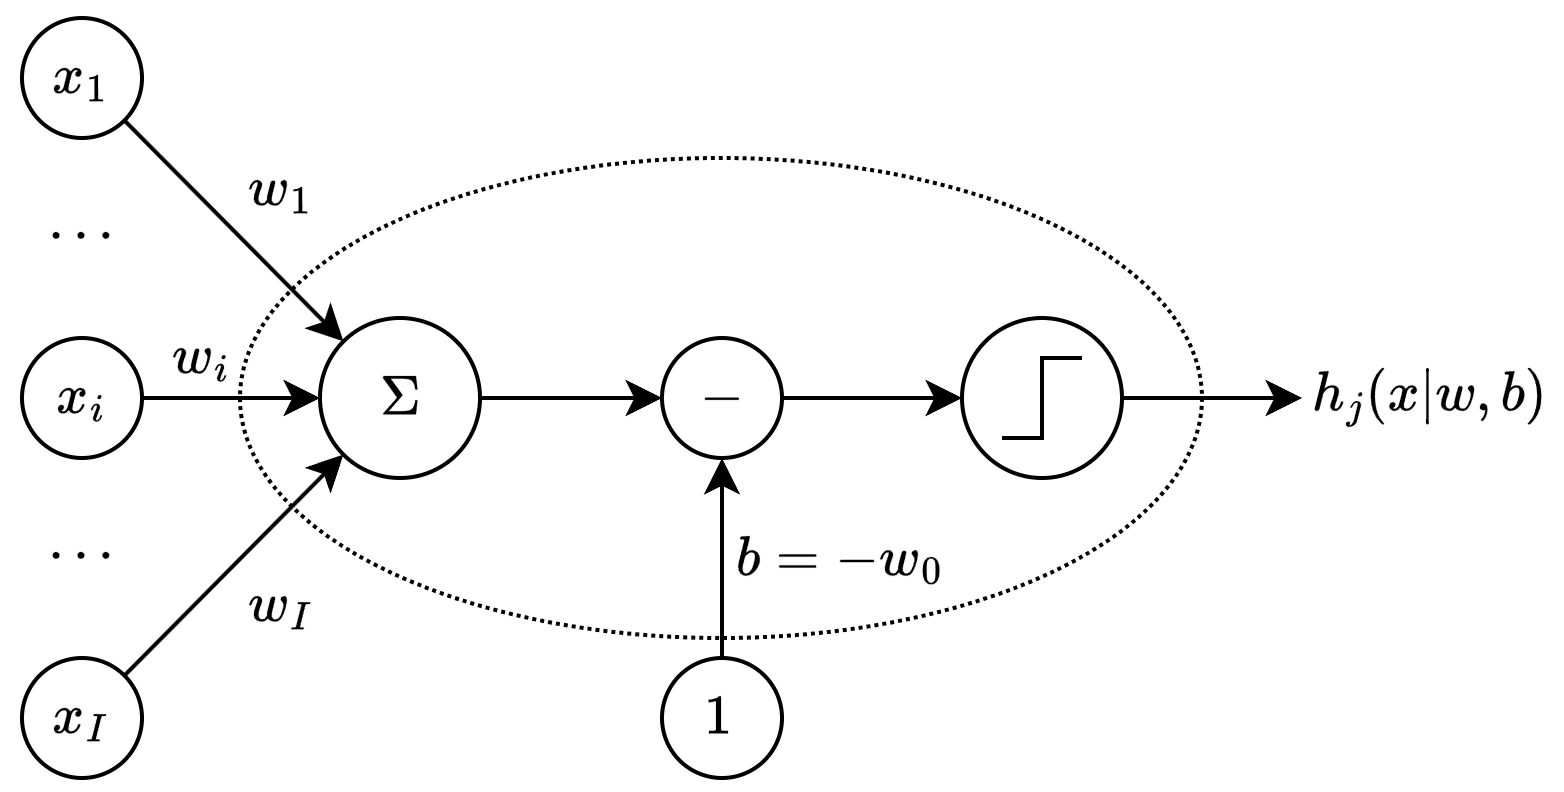
\includegraphics[width=0.75\linewidth]{images/neuron.png}
    \caption{Artificial neuron}
\end{figure}
\noindent The output function $h_j(\mathbf{x}|\mathbf{w},b)$ is given by:
\[h_j(\mathbf{x}|\mathbf{w},b)=h_j\left(\sum_{i=1}^Iw_ix_i-b\right)=h_j\left(\sum_{i=0}^Iw_ix_i\right)=h_j\left(\mathbf{w}^T\mathbf{x}\right)\]
\noindent The activation function in an artificial neuron can take various forms, such as a step function (outputting values between 0 and 1) or a sine function (outputting values between -1 and 1).

The Perceptron computes a weighted sum of its inputs and applies a thresholding function to produce its output:
\[h_j(\mathbf{x}\mid\mathbf{w})=h_j\left(\mathbf{w}^T\mathbf{x}\right)=\text{Sign}(\mathbf{w}^T\mathbf{x})\]
This defines a linear classifier, where the decision boundary is a hyperplane described by:
\[\mathbf{w}^T\mathbf{x}=0\]
The linear decision boundary enables the Perceptron to implement Boolean logic operators. 
However, the Perceptron struggles when data cannot be separated by a linear boundary.
In such cases, additional strategies are necessary. 
These challenges paved the way for more advanced models, such as Multi-Layer Perceptrons.

\paragraph*{Hebbian learning}
Hebbian learning, often summarized by the phrase cells that fire together, wire together, follows these principles:
\begin{enumerate}
    \item Initialize weights randomly.
    \item Adjust weights for each sample (online learning), but only if the sample is misclassified.
\end{enumerate}
The weight update rule is given by:
\[w_i^{k+1}=w_i^k+\eta x_i^kt^k\]
Here, $\eta$ is the learning rate, $x_i^k$ represents the $i$-th input to the Perceptron at time $k$, and $t^k$ is the desired output at the same time. 
    \section{Schedule classification}
Classify the following schedule with respect to CSR and VSR classes:  
\[r_2(u) w_2(s) r_1(x) r_2(y) w_3(y) r_5(x) w_5(u) w_3(s)w_2(u) w_3(x) w_1(u) r_4(y) w_5(z) r_5(z)\]

\paragraph*{Solution}
Since CSR contains VSR we check with the conflict graph. To do so we first divide the schedule based on the resources: 
\begin{itemize}
    \item $x: r_1 \: r_5 \:w_3$
    \item $y: r_2 \: w_3 \:r_4$
    \item $z: w_5 \: r_5$
    \item $s: w_2 \: w_3$
    \item $u: r_2 \: w_5 \: w_2 \:w_1$
\end{itemize}
The nodes are $\{1,2,3,4,5\}$ and the arcs are found with the write-write or write-read relations found in the previous groups. So we have the following graph:
\begin{figure}[H]
    \centering
    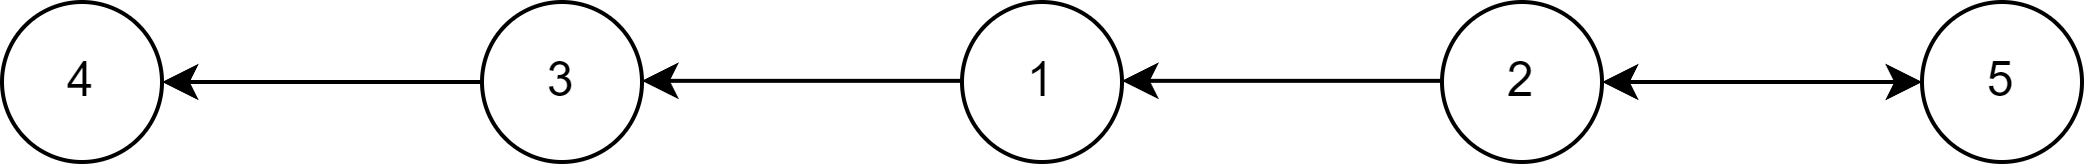
\includegraphics[width=0.5\linewidth]{images/conflictgraph1.png}
\end{figure}
It is possible to see that there is a cycle between two and five. The definition of VSR states that we need to have the same reads-from relations and final writes. So, we try to find a view-equivalent 
schedule that is also CSR. One possible solution is simply to swap the two writes on the resource $u$ and that is sufficient to eliminate the cycle. So, the schedule: 
\[r_2(u) w_2(s) r_1(x) r_2(y) w_3(y) r_5(x) w_5(u) w_2(u) w_3(s) w_3(x) w_1(u) r_4(y) w_5(z) r_5(z)\]
is CSR and also VSR.    

    \chapter{Requirements engineering}
    \section{Introduction}

Sensors serve to detect both the internal condition of the robot (proprioceptive sensors) and the external state of the environment (exteroceptive sensors).

Effectors are responsible for altering the state of the environment, with actuators facilitating the actions of effectors.
    \section{Linear regression}

The goal of regression is to approximate a function $f(x)$ that maps input $x$ to a continuous output $t$ from a dataset $\mathcal{D}$: 
\[\mathcal{D}=\left\{ \left\langle x,t \right\rangle \right\} \implies t=f(x)\]
Here, $x$ is a vector. 
To perform regression, we assume the existence of a function capable of performing this mapping.
The key components of constructing a linear regression problem include:
\begin{itemize}
    \item The method used to model the function $f$ (the hypothesis space). 
    \item The evaluation criteria for the approximation (the loss function).
    \item The optimization process for optimizing the model.
\end{itemize}

In linear regression, the function $f$ is modeled using linear functions. 
This choice is motivated by several factors:
\begin{itemize}
    \item Linear models are easily interpretable, making them suitable for explanation.
    \item Linear regression problems can be solved analytically, allowing for efficient computation.
    \item Linear functions can be extended to model nonlinear relationships.
    \item More sophisticated methods often build upon or incorporate elements of linear regression.
\end{itemize}

\paragraph*{Hypothesis space}
In mathematical terms, the approximation $y$ can be defined as: 
\[y(\textbf{x},\textbf{w})=w_0+\sum_{j=1}^{D-1}w_j x_j=\textbf{w}^T\textbf{x}\]
Here, $\textbf{x} = \left( 1,x_1,\dots,x_{D-1} \right)$ is a vector, and $w_0$ is called the bias parameter.
It's important to note that the output $y$ is a scalar value. 

In a two-dimensional space, our hypothesis space will be the set of all points in the plane $(w_0,w_1)$. 
The coordinates of each point will correspond to a line in the $\left( \textbf{x}, y \right)$ space.

\paragraph*{Loss function}
A commonly used error loss function for the linear regression problem is the sum of squared errors (SSE), defined as:
\[L(\textbf{w})=\dfrac{1}{2}\sum_{n=1}^{N}\left( y(x_n, \textbf{w})-t_n \right)^2\]
This sum is also referred to as the residual sum of squares (RSS) and can be expressed as the sum of squared residual errors:
\[RSS(\textbf{w})=\left\lVert \boldsymbol{\epsilon}^2_2 \right\rVert = \sum_{i=1}^{N}\epsilon^2_i \]
This formulation of the loss function allows for obtaining a closed-form optimization solution.

\paragraph*{Optimization}
For linear models, a closed-form optimization of the RSS, known as least squares, begins with the matrix representation of the loss function:
\[L(\textbf{w})=\dfrac{1}{2}RSS(\textbf{w})=\dfrac{1}{2}\left( \textbf{t}-\boldsymbol{\Phi}_{\textbf{w}} \right)^T\left( \textbf{t}-\boldsymbol{\Phi}_{\textbf{w}} \right)\]
Here, $\boldsymbol{\Phi}=\begin{bmatrix} \phi(x_1) & \dots & \phi(x_N)\end{bmatrix}^T$ and $\textbf{t}=\begin{bmatrix}t_1 & \dots & t_n\end{bmatrix}^T$.
To find the optimal $\textbf{w}$, we compute the first derivative of $L(\textbf{w})$ and set it to zero:
\[\hat{\textbf{w}}_{OLS}=\left( \boldsymbol{\Phi}^T\boldsymbol{\Phi}\right)^{-1}\boldsymbol{\Phi}^T\textbf{t}\]
However, the inversion of the matrix $\boldsymbol{\Phi}^T\boldsymbol{\Phi}^{-1}$ can be computationally expensive, especially for large datasets, with a complexity of $O(nm^2+m^3)$, assuming the matrix is non-singular (invertible). 

To mitigate this, stochastic gradient descent (SGD) can be employed. 
The algorithm known as least mean squares (LMS) uses the following update rule:
\[L(\textbf{x})=\sum_nL(x_n)\]
Expanding this, we get:
\begin{align*}
    \textbf{w}^{(n+1)}  &= \textbf{w}^{(n)}-\alpha^{(n)}\nabla L(x_n) \\
                        &= \textbf{w}^{(n)}-\alpha^{(n)}\left( \textbf{w}^{(n)^T}\phi(\textbf{x}_n)-t_n \right)\phi(\textbf{x}_n)
\end{align*}
Here, $\alpha$ is the learning rate, and convergence is guaranteed if $\sum_{n=0}^{\infty}=+\infty$ and $\sum_{n=0}^{\infty}=\alpha^{(n)^2}<+\infty$.

If the regression problem involves multiple outputs, meaning that $\textbf{t}$ is not a scalar, we can solve each regression problem independently.
However, we can still use the same set of basis functions.
The solution for the weight vectors for all outputs can be expressed as:
\[\hat{\textbf{W}}=\left( \boldsymbol{\Phi}^T\boldsymbol{\Phi}\right)^{-1}\boldsymbol{\Phi}^T\textbf{T}\]
Here, each column of matrix $\textbf{T}$ and $\hat{\textbf{W}}$ corresponds to the target vector and the weight vector for each output, respectively.
This solution can be easily decoupled for each output $k$: 
\[\hat{\textbf{w}}_k=\left( \boldsymbol{\Phi}^T\boldsymbol{\Phi}\right)^{-1}\boldsymbol{\Phi}^T\textbf{t}_k\]
An advantage of this approach is that $\left( \boldsymbol{\Phi}^T\boldsymbol{\Phi}\right)^{-1}$ only needs to be computed once, regardless of the number of outputs.

\subsection{Basis function}
While a linear combination of input variables may not always suffice to model data, we can still construct a regression model that is linear in its parameters. 
This can be achieved by defining a model using non-linear basis functions, expressed as:
\[y(\textbf{x},\textbf{w})=w_0+\sum_{j=1}^{M-1}w_j \phi_j(\textbf{x})=\textbf{w}^T\boldsymbol{\phi}(\textbf{x})\]
Here, the components of the vector  $\boldsymbol{\phi}(\textbf{x})=\left( 1,\phi_1(\textbf{x}),\dots,\phi_{M-1}(\textbf{x}) \right)^T$  are referred to as features.
These features allow for a more flexible representation of the input data, enabling the model to capture non-linear relationships between the input variables and the output.
\begin{example}
    Let's reconsider a set of data regarding individuals' weight and height, along with their completion times for a one-kilometer run:
    \begin{table}[H]
        \centering
        \begin{tabular}{c|c|c}
        \textbf{Height (cm)} & \textbf{Weight (kg)} & \textbf{Completion time (s)} \\ \hline
        180                  & 70                   & 180                          \\
        184                  & 80                   & 220                          \\
        174                  & 60                   & 170                         
        \end{tabular}
    \end{table}
    We can model this problem using a dummy variable and introduce the Body Mass Index (BMI) as a new feature:
    \begin{table}[H]
        \centering
        \begin{tabular}{c|c|c|c|c}
        \textbf{Dummy variable} & \textbf{Height (cm)} & \textbf{Weight (kg)} & \textbf{BMI} & \textbf{Completion time (s)} \\ \hline
        $x_0$                   & $x_1$                & $x_2$                & $x_3$        & $t$                          \\
        1                       & 180                  & 70                   & 21           & 180                          \\
        1                       & 184                  & 80                   & 23           & 220                          \\
        1                       & 174                  & 60                   & 20           & 170                         
        \end{tabular}
    \end{table}
    Here, the dummy variable $x_0$ is always initialized to one.
    Now, we have the option to retain or discard the weight and height variables, considering only the BMI values for analysis.
\end{example}
The most commonly used basis functions in regression are:
\begin{itemize}
    \item \textit{Polynomial}: 
        \[\phi_j(x)=x^j\]
    \item \textit{Gaussian}:
        \[\phi_j(x)=\exp \left( -\dfrac{\left( x-\mu_j \right)^2}{2 \sigma^2} \right) \]
    \item \textit{Sigmoidal}: 
        \[\phi_j(x)=\dfrac{1}{1+\exp\left(\dfrac{\mu_j-x}{\sigma}\right)}\]
\end{itemize}
Here, the constant $\mu_j$ is referred to as a hyperparameter, as its value needs to be determined through experimentation and depends on the user's experience.

\begin{figure}[H]
    \centering
    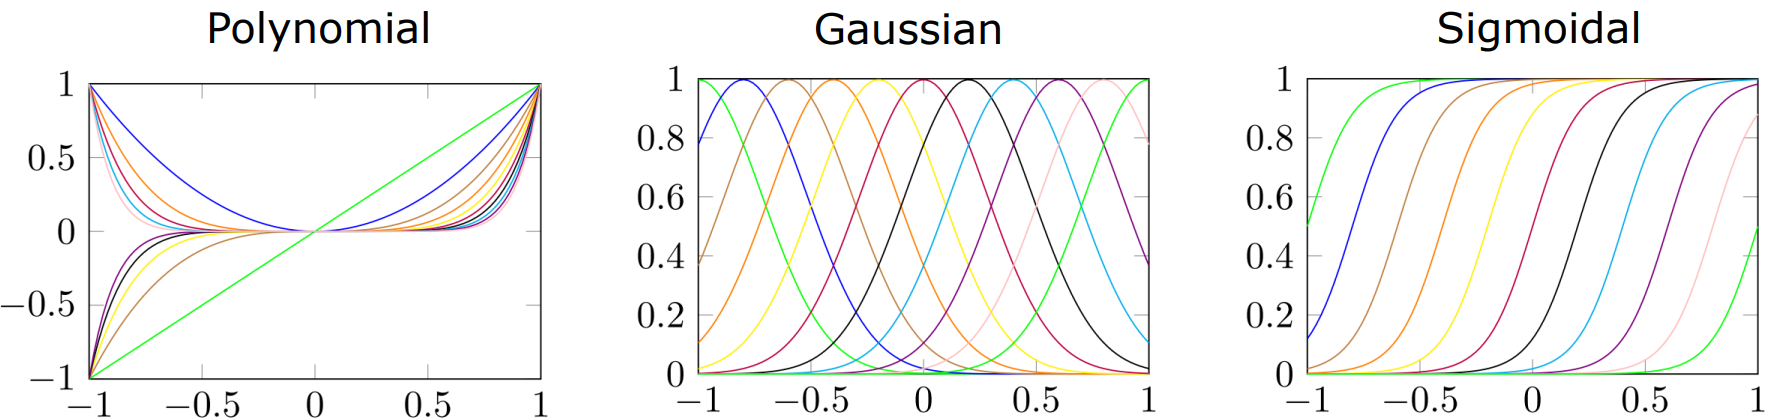
\includegraphics[width=0.75\linewidth]{images/basis.png}
    \caption{Some possible basis functions shapes}
\end{figure}

It's noteworthy that the Gaussian basis function allows for a local approximation by omitting values that are close to zero.
This approach enables capturing the relationship between the input and output in a reduced input space area.
As we move away from the mean, approaching zero, the values become negligible.

\subsection{Regularization}
A function can achieve a better approximation by increasing the degree of the polynomial used in the regression.
\begin{example}
    Consider a function generating a set of points with some noise:
    \begin{figure}[H]
        \centering
        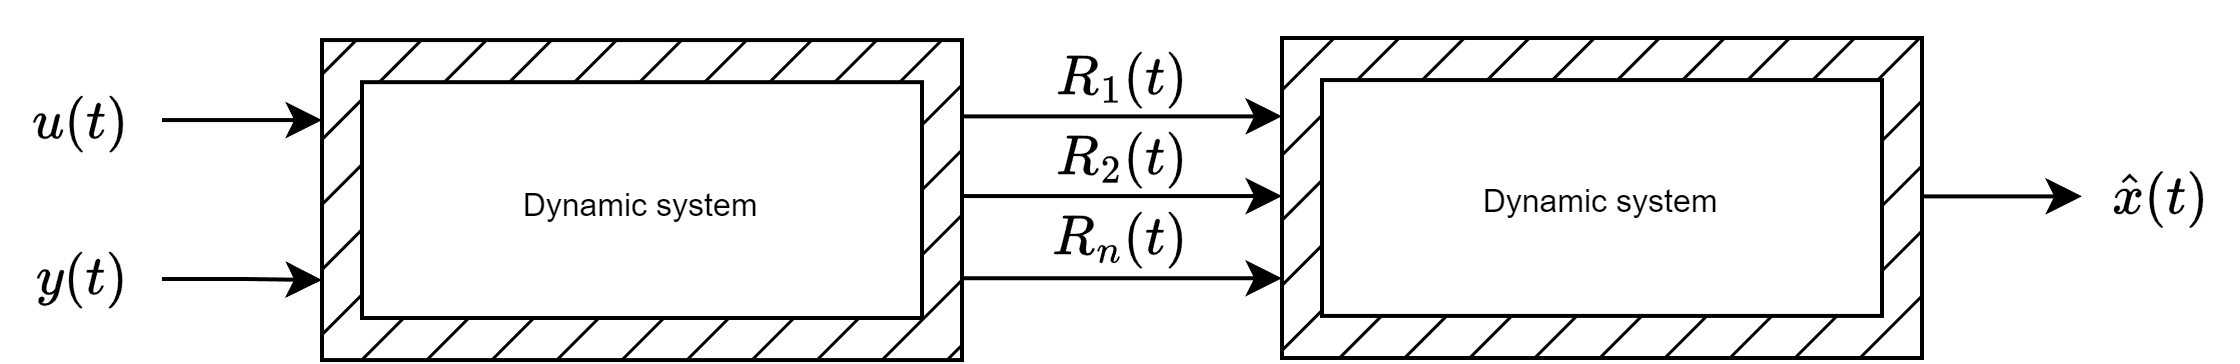
\includegraphics[width=0.25\linewidth]{images/reg.png}
    \end{figure}
    Using a second-order polynomial instead of a linear one provides a better approximation:
    \begin{figure}[H]
        \centering
        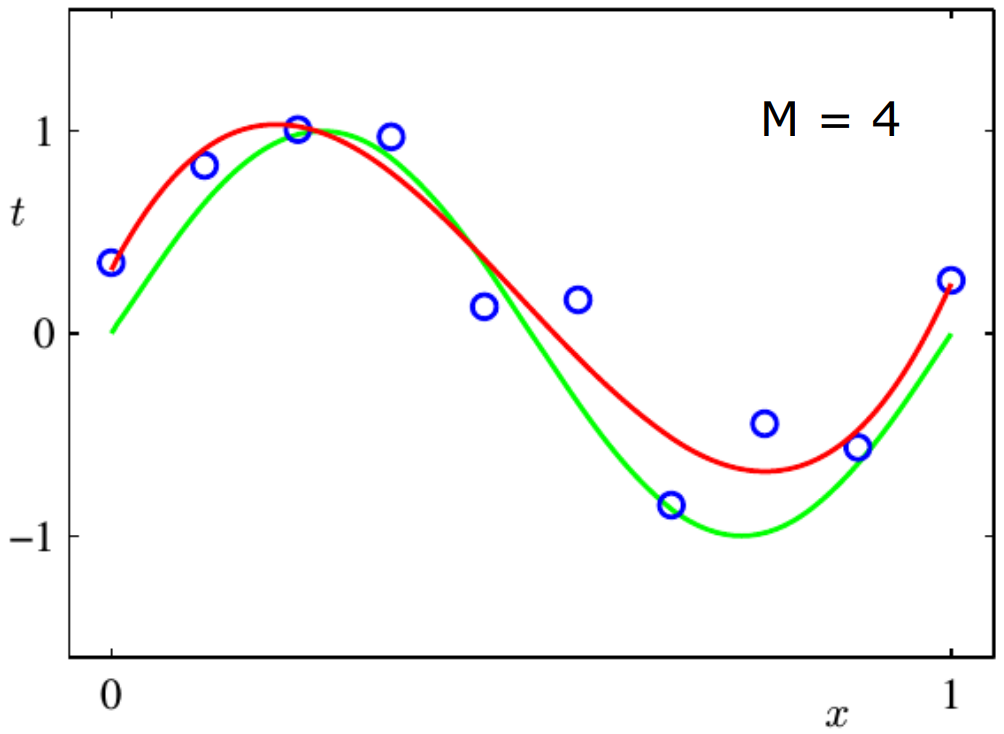
\includegraphics[width=0.25\linewidth]{images/reg1.png}
    \end{figure}
    Further improving the approximation can be achieved with a higher-degree polynomial (e.g., ninth grade):
    \begin{figure}[H]
        \centering
        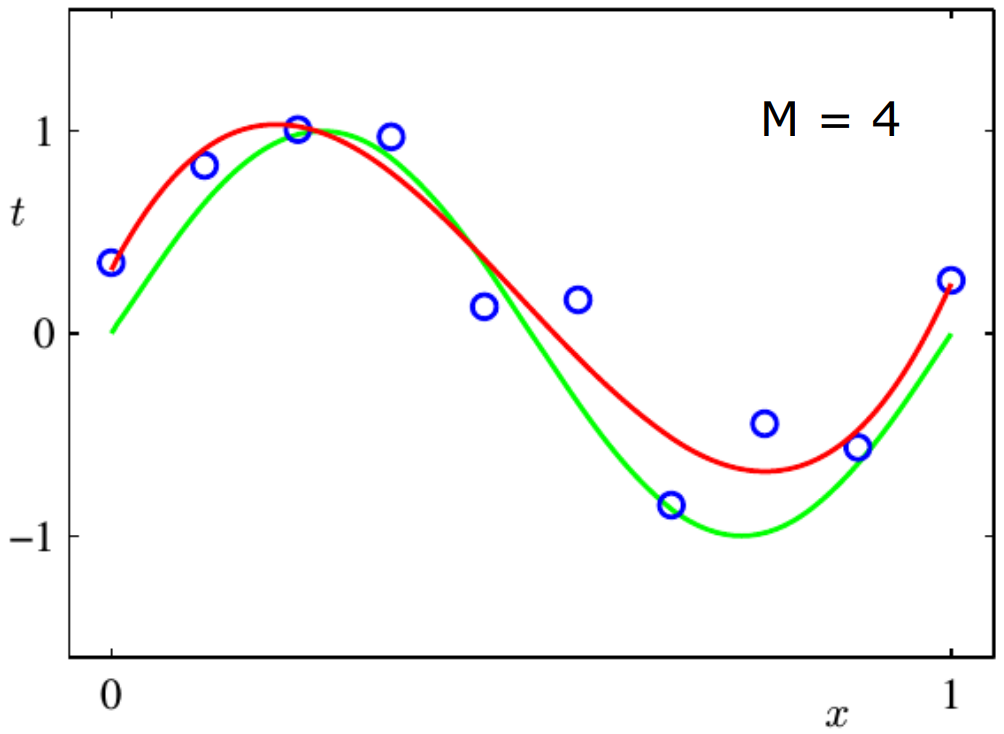
\includegraphics[width=0.25\linewidth]{images/reg1.png}
    \end{figure}
\end{example}
However, increasing the polynomial degree also increases the complexity of the model parameters.
To address this complexity, adjustments are needed in the loss function:
\[L(\textbf{w})=L_D(\textbf{w})+\lambda L_W(\textbf{w})\]
Here, $L_D(\textbf{w})$ represents the usual loss function, $L_W(\textbf{w})$ reflects model complexity (a hyperparameter), and $\lambda$ is the regularization coefficient.
$L_W(\textbf{w})$ can be tailored using ridge regression or lasso methods.

\paragraph*{Ridge regression}
In ridge regression, the regularization term $L_W(\textbf{w})$ is defined as:
\[L_W(\textbf{w})=\dfrac{1}{2}\textbf{w}^T\textbf{w}=\dfrac{1}{2}\left\lVert \textbf{w} \right\rVert_2^2 \]
Thus, the overall loss function becomes:
\[L(\textbf{w})=\dfrac{1}{2}\sum_{i=1}^N \left( t_i-\textbf{w}^T\phi(x_i) \right)^2 + \dfrac{\lambda}{2}\left\lVert \textbf{w} \right\rVert_2^2\]
Despite the regularization term, the loss function remains quadratic with respect to $w$, allowing for closed-form optimization:
\[\hat{\textbf{w}}_{ridge}=\left( \lambda\textbf{I}+\boldsymbol{\Phi}^T \boldsymbol{\Phi} \right)^{-1}\boldsymbol{\Phi}^T\text{t}\]
The term $\lambda\textbf{I}$ is crucial in solving the singularity problem, as it transforms a non-singular matrix into a singular one with an appropriate choice of $\lambda$. 

\paragraph*{Lasso}
Another common regularization method is lasso, where the regularization term $L_W(\textbf{w})$ is defined as:
\[L_W(\textbf{w})=\dfrac{1}{2}\left\lVert \textbf{w} \right\rVert_1=\dfrac{1}{2}\sum_{j=0}^{M-1}\left\lvert w_j \right\rvert\]
Thus, the overall loss function becomes:
\[L(\textbf{w})=\dfrac{1}{2}\sum_{i=1}^N \left( t_i-\textbf{w}^T\phi(x_i) \right)^2 + \dfrac{\lambda}{2}\left\lVert \textbf{w} \right\rVert_1\]
In this case, closed-form optimization is not possible. 
However, lasso typically leads to sparse regression models: when the regularization coefficient $\lambda$ is large enough, some components of $\hat{\textbf{w}}$ become equal to zero.
Regularization can be seen as equivalent to minimizing  $L_D(\textbf{w})$ subject to the constraint:
\[\sum_{j=0}^{M-1}\left\lvert w_j \right\rvert \leq \eta\] 

\subsection{Linear regression with probability}
We can approach regression in a probabilistic manner by defining a model that probabilistically maps inputs ($x$) to outputs ($t$).
This model, denoted as $y(x, w)$, incorporates unknown parameters ($w$).
We then model the likelihood, i.e., the probability that observed data $\mathcal{D}$ is generated by a given set of parameters ($w$), as: 
\[\text{P}(\mathcal{D}|\textbf{w})\]
Finally, we estimate the parameters ($w$) by maximizing the likelihood:
\[\textbf{w}_{ML}=\argmax_{\textbf{w}}\text{P}(\mathcal{D}|\textbf{w})\]

For linear regression, we define the model as:
\[t=y(\textbf{x},\textbf{w})+\epsilon=\textbf{w}^T\boldsymbol{\Phi}(\textbf{x})+\epsilon\]
Here, we assume a linear model for $y(\textbf{x},\textbf{w})$ and introduce noise  $\epsilon\sim\mathcal{N}(0,\sigma^2)$. 
Consequently, given a dataset $\mathcal{D}$ of $N$ samples with inputs $\textbf{X}=\begin{bmatrix}\textbf{x}_1 & \dots & \textbf{x}_n \end{bmatrix}$ and outputs $\textbf{t}=\begin{bmatrix}t_1 & \dots & t_n \end{bmatrix}^T$, we have: 
\[\text{P}(\mathcal{D}|\textbf{w})=\text{P}(\textbf{t}|\textbf{X},\textbf{w},\sigma^2)=\prod_{n=1}^{N}\mathcal{N}(t_n|\textbf{w}^T\boldsymbol{\Phi}(\textbf{x}_n),\sigma^2)\]
 
To find $\textbf{w}_{ML}$, it is convenient to maximize the log-likelihood, obtaining:
\[\ell (\textbf{w})=\ln\text{P}(t_n|\textbf{x}_n, \textbf{w} ,\sigma^2)=-\dfrac{N}{2}\ln(2\pi\sigma^2)-\dfrac{1}{2\sigma^2}RSS(\textbf{w})\]
Notice that the first part of the final formula is a constant independent of $\textbf{w}$, so it can be ignored in maximizing the likelihood.
Solving the optimization problem by setting the gradient to zero $\ell (\textbf{w})=0$, yields the final formula:
\[\textbf{w}_{ML}=\left( \boldsymbol{\Phi}^T\boldsymbol{\Phi} \right)^{-1}\boldsymbol{\Phi}^T\textbf{t}\]
This result aligns with the ordinary least squares approach.

This outcome allows us to interpret ordinary least squares from a probabilistic perspective, confirming that we are utilizing a normally distributed probabilistic function to generate the residuals in OLS.

\paragraph*{Bayesian linear regression}
Bayesian linear regression follows a structured approach:
\begin{enumerate}
    \item Formulation of probabilistic knowledge:
        \begin{enumerate}
            \item Qualitatively define the model expressing our knowledge.
            \item Incorporate unknown parameters into the model.
            \item Represent assumptions about these parameters with a prior distribution before observing any data.
        \end{enumerate}
    \item Data observation.
    \item Computation of posterior probability distribution for parameters:
        \[\text{P}(parameters|data)=\dfrac{\text{P}(data|parameters)\text{P}(parameters)}{\text{P}(data)}\]
    \item Utilization of Posterior Distribution to:
        \begin{itemize}
            \item Make predictions by averaging over the posterior distribution.
            \item Assess or accommodate uncertainty in parameter values.
            \item Make decisions by minimizing expected posterior loss.
        \end{itemize}
\end{enumerate}

The posterior distribution for model parameters is derived by combining the prior with the likelihood for parameters given the data:
\[\text{P}(\textbf{w}|\mathcal{D})=\dfrac{\text{P}(\mathcal{D}|\textbf{w})\text{P}(\textbf{w})}{\text{P}(\mathcal{D})}\]
Here, $\text{P}(\textbf{w})$ represents the prior probability over parameters, $\text{P}(\mathcal{D}|\textbf{w})$ denotes the likelihood, and $\text{P}(\mathcal{D})$ is the marginal likelihood acting as a normalization constant: 
\[\text{P}(\mathcal{D})=\int\text{P}(\mathcal{D}|\textbf{w})\text{P}(\textbf{w})d\textbf{w}\] 

The mode of the posterior, known as the Maximum A Posteriori (MAP) estimate, yields the most probable value of $\textbf{w}$ given the data.

A Gaussian likelihood assumption allows the prior to be modeled conveniently as a conjugate prior:
\[\text{P}(\textbf{w})=\mathcal{N}(\textbf{w}|\textbf{w}_0,\textbf{S}_0)\]
Consequently, the posterior remains Gaussian:
\[\text{P}(\textbf{w}|\textbf{t},\boldsymbol{\Phi},\sigma^2)\varpropto \mathcal{N}(\textbf{w}|\textbf{w}_0,\textbf{S}_0)\mathcal{N}(\textbf{t}|\boldsymbol{\Phi}\textbf{w},\sigma^2\textbf{I})\]
Resulting in:
\[\begin{cases}
    \text{P}(\textbf{w}|\textbf{t},\boldsymbol{\Phi},\sigma^2)=\mathcal{N}(\textbf{w}|\textbf{w}_N,\textbf{S}_N) \\
    \textbf{w}_N=\textbf{S}_N\left(\textbf{S}_0^{-1}\textbf{w}_0+\dfrac{\boldsymbol{\Phi}^T\textbf{t}}{\sigma^2}\right) \\
    \textbf{S}_N^{-1}=\textbf{S}_0^{-1}+\dfrac{\boldsymbol{\Phi}^T\boldsymbol{\Phi}}{\sigma^2}
\end{cases}\]

\paragraph*{Prior infinitely broad}
When the prior distribution is infinitely broad, the Maximum A Posteriori (MAP) estimate coincides with the Maximum Likelihood (ML) solution:
\[\begin{cases}
    \lim_{\textbf{S}_0\rightarrow\infty}\textbf{w}_N=\left( \boldsymbol{\Phi}^T\boldsymbol{\Phi} \right)^{-1}\boldsymbol{\Phi}^T\textbf{t} \\
    \lim_{\textbf{S}_0\rightarrow\infty}\textbf{S}_N^{-1}=\dfrac{\boldsymbol{\Phi}^T\boldsymbol{\Phi}}{\sigma^2}
\end{cases}\]
This yields the ordinary least squares formula.
However, in this case, we also have the covariance matrix, providing information about the related uncertainty.
The only missing parameter is $\sigma^2$, which can be computed as:
\[\sigma^2=\dfrac{1}{N-M}\sum_{n=1}^{N}\left( t_n-\hat{\textbf{w}}^T\boldsymbol(\phi)(\textbf{x}_n) \right)^2\]
The ML estimate $\textbf{w}_{ML}$ of $\textbf{w}$ has the smallest variance among linear unbiased estimates and the lowest Mean Squared Error (MSE) among linear unbiased estimates (Gauss-Markov).

\paragraph*{Prior not infinitely broad}
When the prior distribution is not infinitely broad, such that $\textbf{w}_0=0$ and $\textbf{S}_0=\tau^2\textbf{I}$, we can express the logarithm of the posterior distribution $\text{P}(\textbf{w}|\textbf{t})$ as:
\[\ln\text{P}(\textbf{w}|\textbf{t})=-\dfrac{1}{2\sigma^2}\sum_{i=1}^{N}\left(t_i-\textbf{w}^T\boldsymbol{\phi}(\textbf{x}_i)\right)^2-\dfrac{1}{2\tau^2}\left\lVert \textbf{w}\right\rVert_2^2 \]
In this scenario, the Maximum A Posteriori estimate, MAP($\textbf{w}N$), coincides with the solution of ridge regression $\hat{\textbf{w}}{ridge}$ with a regularization parameter $\lambda$ set to $\lambda=\frac{\sigma^2}{\tau^2}$.

\paragraph*{Sequential learning}
How to leverage the Bayesian approach for sequential learning:
\begin{enumerate}
    \item Begin by computing the posterior with the initial data.
    \item As additional data becomes available, update the prior with this new information to obtain the updated posterior.
\end{enumerate}

\paragraph*{Predictive distribution}
In a Bayesian framework, one can determine the probability distribution of the target variable for a new sample $\textbf{x}^\ast$ (given the training data $\mathcal{D}$) by integrating over the posterior distribution:
\[\text{P}(t^\ast|\textbf{x}^\ast,\mathcal{D})=\mathbb{E}\left[ t^\ast|\textbf{x}^\ast,\textbf{w},\mathcal{D} \right] = \int\text{P}(t^\ast|\textbf{x}^\ast,\textbf{w},\mathcal{D})\text{P}(\textbf{w}|\mathcal{D})d\textbf{w}\]
This is commonly referred to as the predictive distribution.
However, computing this predictive distribution typically involves the intractable task of determining the posterior distribution.
Nevertheless, under certain assumptions, it is possible to compute the predictive distribution as follows: 
\[\sigma_N^2(\textbf{x})=\sigma^2+\boldsymbol{\phi}(\textbf{x})^T\textbf{S}_N\boldsymbol{\phi}(\textbf{x})\]
Here, as the number of data points $N$ approaches infinity, the uncertainty associated with the parameters (second term) diminishes, and the variance of the predictive distribution depends solely on the variance of the data ($\sigma^2$). 

\subsection{Challenges and limitations}
Modeling presents challenges in ensuring our model effectively represents a wide range of plausible functions while maintaining informative priors without overly spreading out probabilities or assigning negligible values.

On the computational side, limitations arise with analytical integration, particularly in cases involving non-conjugate priors and complex models. 
Approaches like Gaussian (Laplace) approximation, Monte Carlo integration, and variational approximation become necessary for addressing these complexities and achieving accurate results.

Linear models with fixed basis functions offer several benefits:
\begin{itemize}
    \item They permit closed-form solutions, facilitating efficient computation.
    \item They lend themselves to tractable Bayesian treatment, enabling principled uncertainty quantification.
    \item They can capture non-linear relationships by employing appropriate basis functions.
\end{itemize}
However, these models also come with several drawbacks:
\begin{itemize}
    \item Basis functions remain static and non-adaptive to variations in the training data.
    \item These models are susceptible to the curse of dimensionality, particularly when dealing with high-dimensional feature spaces.
\end{itemize}
    \section{Classification}














    \section{Multiple scanners}

Sometimes is useful to have more than one scanner together. 
To facilitate the support for multiple scanners, the following methods are employed:
\begin{itemize}
    \item Rules can be designated with the name of the associated scanner, known as the start condition.
    \item Special actions enable the transition between scanners.
\end{itemize}

A start condition, denoted by \texttt{S} is utilized to annotate rules as \texttt{<S>RULE} and activate rules when the scanner operates in the \texttt{S} start condition.
Start conditions can be:
\begin{itemize}
    \item \textit{Exclusive}, declared with \texttt{$\%$x S}; this disables unmarked rules when the scanner operates in the \texttt{S} start condition.
    \item \textit{Inclusive}, declared with \texttt{$\%$s S}; unmarked rules are active when the scanner operates in the \texttt{S} start condition.
\end{itemize}
The initial condition is inclusive by default.
Additionally:
\begin{itemize}
    \item The \texttt{*} start condition matches any start condition.
    \item The initial start condition is denoted as \texttt{INITIAL}.
    \item Start conditions are represented as integers.
    \item The current start condition is stored in the \texttt{YY$\_$START} variable.
\end{itemize}  
    \section{Skyline queries}

Skyline queries aim to identify superior objects across multiple perspectives, relying on the concept of dominance.
\begin{definition}[\textit{Domination}]
    A tuple $t$ dominates a tuple $s$ ($t \prec s$) if and only if $t$ in nowhere worse than $s$: 
    \[\forall i, 1 \leq i \leq m \rightarrow t[A_i] \leq s[A_i]\] 
    And is better at least once: 
    \[\exists j, 1 \leq j \leq m \land t[A_j] < s[A_j]\]
\end{definition}
\begin{definition}[\textit{Skyline}]    
    The skyline of a relation is the set of its non-dominated tuples.
\end{definition}

The convention on the skyline queries is that lower values are better than higher values.
The convention is that lower values are considered better. 
A tuple is part of the skyline if it is the top-1 result with respect to at least one monotone scoring function. 

\paragraph*{Query syntax}
The syntax for skyline queries can be expressed as follows:
\begin{lstlisting}[style=SQL]
SELECT <attributes>
FROM R1,R2,...,Rn
WHERE <conditions>
GROUP BY <conditions>
HAVING <conditions>
SKYLINE OF [DISTINCT] d1[MIN|MAX|DIFF], ..., dm[MIN|MAX|DIFF]
ORDER BY <conditions>
\end{lstlisting}
This query can be easily translated into a standard query, but the result is too slow and cannot be used in practice. 

\subsection{Block Nested Loop algorithm}
The Block Nested Loop algorithm takes a dataset $D$ of multidimensional points as input and outputs the skyline of $D$. 
Its complexity is $O(n^2)$, making it inefficient for large datasets.
\begin{algorithm}[H]
    \caption{Block nested loop algorithm}
        \begin{algorithmic}[1]
            \State $W \leftarrow \varnothing$
            \For {every point $p$ in $D$}
                \If {$p$ not dominated by any point in $W$}
                    \State remove from $W$ the points dominated by $p$
                    \State add $p$ to $W$
                \EndIf
            \EndFor
            \State \Return $W$
        \end{algorithmic}
\end{algorithm}

\subsection{Sort Filter Skyline algorithm}
The Sort Filter Skyline algorithm also takes a dataset $D$ of multidimensional points as input and outputs the skyline of $D$. 
It performs better than the Block Nested Loop algorithm, especially for large datasets, but still has a complexity of $O(n^2)$.
\begin{algorithm}[H]
    \caption{Sort filter skyline algorithm}
        \begin{algorithmic}[1]
            \State $S \leftarrow D$
            \State $W \leftarrow \varnothing$
            \For {every point $p$ in $S$}
                \If {$p$ not dominated by any point in $W$}
                    \State add $p$ to $W$
                \EndIf
            \EndFor
            \State \Return $W$
        \end{algorithmic}
\end{algorithm}
\begin{example}
    Consider the following unordered dataset: 
    \begin{table}[H]
        \centering
        \begin{tabular}{lcc}
        \textbf{Name}                 & \textbf{Cost} & \textbf{Complaints} \\ \hline
        \multicolumn{1}{l|}{Crillon}  & 0.25  & 0.1        \\
        \multicolumn{1}{l|}{Ibis}     & 0.08  & 0.3        \\
        \multicolumn{1}{l|}{Hilton}   & 0.175 & 0.3        \\
        \multicolumn{1}{l|}{Sheraton} & 0.2   & 0.2        \\
        \multicolumn{1}{l|}{Novotel}  & 0.15  & 0.1       
        \end{tabular}
    \end{table}
    The skyline, consisting of Novotel and Ibis, is identified by the algorithm.
\end{example}

\subsection{Summary}
Skyline queries are effective in identifying potentially interesting objects when user preferences are unknown. 
They are simple to use but return a large number of objects, and their computation is not highly efficient. 
Skyline queries are agnostic with respect to user preferences.

\paragraph*{K-skyband} 
To enhance skyline queries, the concept of $k$-skyband is introduced, where the result includes a set of tuples dominated by fewer than $k$ tuples.
    \section{ARMA process}

We can define a process that combines elements from both the AutoRegressive and Moving Average processes as follows:
\[y(t)=a_1y(t-1)+a_2y(t-2)+\cdots+a_m y(t-m)+c_0e(t)+c_1e(t-1)+\cdots+c_n e(t-n) \]
Here, $e(t)\sim WN(0,\lambda^2)$.

This process comprises two components: one being the AR($m$) process and the other being the MA($n$) process. 
It is denoted as an ARMA($m,n$) process.
Since it combines elements from two distinct processes, we can make the following observations:
\begin{itemize}
    \item The MA($n$) process is equivalent to an ARMA($0,n$) process.
    \item The AR($m$) process is equivalent to an ARMA($m,0$) process. 
\end{itemize}
\begin{figure}[H]
    \centering
    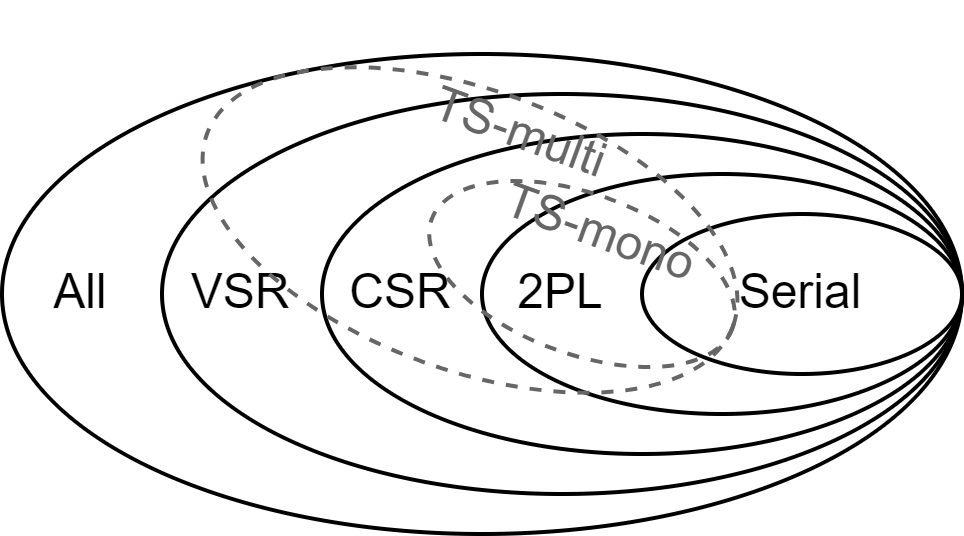
\includegraphics[width=0.45\linewidth]{images/set.png}
    \caption{Inclusion of ARMA processes}
\end{figure}

\subsection{Operatorial representation}
Given an ARMA($m,n$) process defined as:
\[y(t)=a_1y(t-1)+a_2y(t-2)+\cdots+a_m y(t-m)+c_0e(t)+c_1e(t-1)+\cdots+c_n e(t-n)\]
Here, $e(t)\sim WN(0,\lambda^2)$.

We can rewrite it using operatorial representation as:
\[y(t)=a_1z^{-1}y(t)+a_2z^{-2}y(t)+\cdots+a_m z^{-m}y(t)+c_0e(t)+c_1z^{-1}e(t)+\cdots+c_n z^{-n}e(t)\]
Rearranging terms, we get:
\[\left(1- a_1z^{-1}-a_2z^{-2}-\cdots-a_m z^{-m}\right)y(t)=\left(c_0+c_1z^{-1}+\cdots+c_n z^{-n}\right)e(t)\]
Finally, we can express $y(t)$ in terms of $e(t)$ using the transfer function notation:
\[y(t)=\dfrac{c_0+c_1z^{-1}+\cdots+c_n z^{-n}}{1- a_1z^{-1}-a_2z^{-2}-\cdots-a_m z^{-m}}e(t)=\dfrac{C(z)}{A(z)}e(t)\]
Here, $C(z)$ and $A(z)$ are polynomials representing the coefficients of the Moving Average and AR parts, respectively. 
This ratio, denoted as $W(z)$, is a discrete-time transfer function. 
This operator acts as a digital filter, transforming the input noise sequence $e(t)$ into the output sequence $y(t)$.

\subsection{Mean value}
Given an ARMA($m,n$) model defined as:
\[y(t)=a_1y(t-1)+a_2y(t-2)+\cdots+a_m y(t-m)+c_0e(t)+c_1e(t-1)+\cdots+c_n e(t-n)\]
where $e(t)\sim WN(0,\lambda^2)$, we can compute its mean as follows:
\begin{align*}
    \mathbb{E}\left[y(t)\right] &= \mathbb{E}\left[a_1y(t-1)+\cdots+a_m y(t-m)+c_0e(t)+\cdots+c_n e(t-n)\right] \\
                                &= a_1\mathbb{E}\left[y(t-1)\right]+\cdots+a_m\mathbb{E}\left[y(t-m)\right] +c_0\underbrace{\mathbb{E}\left[e(t)\right]}_0 +\cdots+c_n\underbrace{\mathbb{E}\left[e(t-n)\right]}_0
\end{align*}
Under the assumption that $a_1,a_2,\dots,a_m$ are chosen such that $y(t)$ constitutes a stationary stochastic process, thus exhibiting a constant mean value, we can simplify the above to:
\[m_y=a_1m_y+a_2m_y+\cdots+a_m m_y \rightarrow m_y=0\]

\subsection{Covariance function}
Given an ARMA($m,n$) model defined as:
\[y(t)=a_1y(t-1)+a_2y(t-2)+\cdots+a_m y(t-m)+c_0e(t)+c_1e(t-1)+\cdots+c_n e(t-n)\]
where $e(t)\sim WN(0,\lambda^2)$, we aim to compute the covariance function at $\tau=0$, considering $m_y=0$:
\begin{align*}
    \gamma_y(0) &=\mathbb{E}\left[ \left(y(t)-m_y\right)\left(y(t)-m_y\right) \right] \\
                &=\mathbb{E}\left[ {\left(y(t)\right)}^2 \right] \\
                &=\mathbb{E}\left[ {\left(a_1y(t-1)+\cdots+a_m y(t-m)+c_0e(t)+\cdots+c_n e(t-n)\right)}^2 \right] \\      
                &=a_1^2\underbrace{\mathbb{E}\left[ {y(t-1)}^2 \right]}_{\gamma_y(0)} +\cdots+c_0^2\underbrace{\mathbb{E}\left[ {e(t)}^2 \right]}_{\lambda^2} +\cdots+c_n^2 \underbrace{\mathbb{E}\left[ {e(t-n)}^2 \right]}_{\lambda^2}  +\\
                &+ 2a_1a_2\underbrace{\mathbb{E}\left[ y(t-1)y(t-2) \right]}_{\gamma_y(1)}  + \cdots + 2a_1c_0\underbrace{\mathbb{E}\left[ y(t-1)e(t) \right]}_{0 \text{ if the times are different}}  + \cdots + 2c_0c_1\underbrace{\mathbb{E}\left[ e(t)e(t-1) \right]}_0  \\   
                &=a_1^2\gamma_y(0) +\cdots+c_0^2\lambda^2 +\cdots+c_n^2 \lambda^2  + 2a_1a_2\gamma_y(1)  + \cdots + 2a_1c_1\mathbb{E}\left[ y(t-1)e(t-1) \right]+\dots    
\end{align*}
We require $\gamma_y(1),\gamma_y(2),\dots,\gamma_y(n)$ to compute $\gamma_y(0)$.

To compute the covariance function at $\tau=1$, considering $m_y=0$, we have:
\begin{align*}
    \gamma_y(1) &=\mathbb{E}\left[ \left(y(t)-m_y\right)\left(y(t-1)-m_y\right) \right] \\
                &=\mathbb{E}\left[ \left(a_1y(t-1)+\cdots+a_m y(t-m)+c_0e(t)+\cdots+c_n e(t-n)\right)y(t-1) \right] \\
                &=a_1\mathbb{E}\left[{y(t-1)}^2\right]+\cdots+c_0\mathbb{E}\left[e(t)y(t-1)\right]+\dots \\
                &=a_1\gamma_y(0)+\cdots+c_0\mathbb{E}\left[e(t)y(t-1)\right]+\dots
\end{align*}
Proceeding with increasing values of $\tau$, we obtain a set of $m$ recursive equations known as Yule-Walker equations for an ARMA($m,n$) process:
\[\begin{cases}
    \gamma_y(0)=a_1^2\gamma_y(0) +a_2^2\gamma_y(0) +2a_1a_2\gamma_y(1) +\dots \\
    \gamma_y(1)=a_1\gamma_y(0) +c_0\mathbb{E}\left[e(t)y(t-1)\right] +\dots \\
    \vdots \\
    \gamma_y(m-1)=a_1\gamma_y(m-2)+\dots
\end{cases}\]
At the end we get a set of $m$ recursive equations called Yule-Walker equations for an ARMA($m,n$) process.
These equations require all covariances $\gamma_y(0),\gamma_y(1),\dots,\gamma_y(m-1)$ to compute $\gamma_y(m)$.
    \section{Parallel projections}

Parallel projections are a type of graphical projection where all projection lines are parallel to each other, resulting in objects appearing the same size regardless of their distance from the observer. 
In parallel projections, the projection plane is positioned perpendicular to the line of sight, and there is no foreshortening or perspective distortion.

\subsection{Orthogonal projections}
Orthogonal projections are characterized by projecting onto planes that align with the $xy$, $yz$, or $zx$ planes, with the projection rays perpendicular to these planes. 
They find primary use in technical drawings, as segments of equal length parallel to an axis retain their identical properties.

It's important to recognize that each plane has two distinct projection directions, resulting in differing orderings of the $z$-component of normalized screen coordinates. 
This can sometimes produce entirely different images.

We'll initially focus on a projection plane corresponding to the $xy$-plane, which is perpendicular to the $z$-axis.
In this setup, visible objects possess negative values in their $z$ coordinate.

The screen boundaries naturally constrain the portion of the 3D world visible on a screen along the horizontal and vertical axes. 
However, it's also necessary to limit the range of a scene along the depth axis for several reasons:
\begin{enumerate}
    \item Prevent displaying objects behind the observer.
    \item Avoid showing objects that are excessively distant from the viewer's perspective.
    \item Enable the $z$-axis of the normalized screen coordinates to be confined within the $0$ to $+1$ range.
\end{enumerate}
These constraints define two planes:
\begin{itemize}
    \item The plane with the closest $z$-component (maximum signed value, minimum absolute value) is termed the near plane.
    \item The one with the farthest $z$-component (minimum signed value, maximum absolute value) is referred to as the far plane.
\end{itemize}
After projection, only points contained within the box bounded by the left, right, top, and bottom screen borders, as well as the near and far planes along the depth axis, can be visualized.
Normalized Screen Coordinates are defined such that the near plane, the left side, and the bottom side of the screen are projected to $z_n=0$, $x_l=-1$, and $y_t=-1$, respectively. 
Conversely, the far plane, the right side, and the top side are projected to $z_f=1$, $x_r=1$, and $y_b=1$, respectively.

\paragraph*{Orthogonal projection matrix}
Orthogonal projections can be implemented by normalizing the $x, y, z$ coordinates of the projection box within the ranges $(-1,1)$, $(-1,1)$, and $(0,1)$ respectively. 
This normalization process, starting from a valid coordinate, can be achieved by multiplying with a suitable matrix.
In particular, we define the projection matrix, $P_{ort}$, as the matrix that, when multiplied with a world coordinate $p_W$, computes the corresponding normalized screen coordinate $p_N$: 
\[P_N=P_{ort}\cdot P_W\]
To obtain normalized coordinates, we must determine the coordinates of the screen borders in 3D space.
We denote $l$ and $r$ as the x-coordinates in 3D space corresponding to locations displayed on the left and right borders of the screen. 
Anything to the left of $l$ will be excluded from the screen, and nothing to the right of $r$ will be visualized. 
Similarly, we use $t$ and $b$ for the $y$-coordinates of the top and bottom borders of the screen in 3D space.
$P_{ort}$
We also denote $-n$ and $-f$ as the $z$-coordinates of the near and far planes in 3D space. 
Since the $z$-axis is oriented opposite to the viewer's perspective, positive distances $n$ and $f$ are generally preferred over negative coordinates where the two planes intersect.

The orthogonal projection matrix $P_{ort}$ is computed in three steps. 
First, we translate the center of the projection box to the near plane at the origin using a translation $T_{ort}$:
\[T_{ort}=\begin{bmatrix}
    1 & 0 & 0 & -\frac{r+l}{2} \\ 
    0 & 1 & 0 & -\frac{t+b}{2} \\ 
    0 & 0 & 1 & -(-n) \\ 
    0 & 0 & 0 & 1 
\end{bmatrix}\]
The second step involves normalizing the coordinates between $-1$ and $1$ (for the $x$-axis and $y$-axis) or 0 and 1 (for the $z$-axis) through a scale transformation $S_{ort}$:
\[S_{ort}=\begin{bmatrix}
    \frac{2}{r-l} & 0 & 0 & 0 \\ 
    0 & \frac{2}{t-b} & 0 & 0 \\ 
    0 & 0 & \frac{1}{f-n} & 0 \\ 
    0 & 0 & 0 & 1 
\end{bmatrix}\]
The last step corrects the direction of the axes with the mirror matrix $M_{ort}$, by inverting the $y$-axis and $z$-axis:
\[M_{ort}=\begin{bmatrix}
    1 & 0 & 0 & 0 \\ 
    0 & -1 & 0 & 0 \\ 
    0 & 0 & -1 & 0 \\ 
    0 & 0 & 0 & 1 
\end{bmatrix}\]
By applying the composition of transformations, we can define the orthogonal projection matrix $P_{ort}$ as follows:
\[M_{ort}=M_{ort}\cdot S_{ort} \cdot T_{ort}=\begin{bmatrix}
    \frac{2}{r-l} & 0 & 0 & \frac{r+l}{l-r} \\ 
    0 & \frac{2}{b-t} & 0 & \frac{t+b}{t-b} \\ 
    0 & 0 & \frac{1}{n-f} & \frac{n}{n-f} \\ 
    0 & 0 & 0 & 1 
\end{bmatrix}\]

\subsection{Aspect ratio}
The ratio between the horizontal and vertical dimensions of the physical screen is known as the aspect ratio: 
\[a=\dfrac{D_x}{D_y}\]
In this definition, the measures for the horizontal and vertical sizes, $D_x$ and $D_y$, are specified in metric units rather than pixels. 
When pixels are square, both metric units and pixels yield the same outcome. 
However, if pixels are not square, only the actual display proportions can ensure images are not distorted.

Normalized screen coordinates do not incorporate the aspect ratio. 
Instead, the projection matrix adjusts for this factor, appropriately scaling the images to ensure they appear with the correct proportions.

To generate images with accurate proportions, the values of $l$, $r$, $t$, and $b$ must be consistent with the aspect ratio $a$ of the monitor: 
\[a=\dfrac{r-l}{t-b}\rightarrow r-l=a\cdot (t-b)\]
In many cases, the projection box is centered at the origin both horizontally and vertically. 
When this occurs, only the half-width of the box $w$, the near plane $n$, the far plane $f$, and the aspect ratio $a$ are required.
\[\begin{cases}
    l=-w \\
    r=w \\
    t=\frac{w}{a} \\
    b=-\frac{w}{a}
\end{cases}\]
As a result the transformation matrix becomes: 
\[P_{ort}=\begin{bmatrix}
    \frac{1}{w} & 0 & 0 & 0 \\ 
    0 & -\frac{a}{w} & 0 & 0 \\ 
    0 & 0 & \frac{1}{n-f} & \frac{n}{n-f} \\ 
    0 & 0 & 0 & 1 
\end{bmatrix}\]

For orthogonal projections where the near plane is positioned at $n=0$, the projection matrix can be further simplified into a non-uniform scaling matrix with factors $S(\frac{1}{w}, -\frac{a}{w}, -\frac{1}{f})$:
\[P_{ort}=\begin{bmatrix}
    \frac{1}{w} & 0 & 0 & 0 \\ 
    0 & -\frac{a}{w} & 0 & 0 \\ 
    0 & 0 & -\frac{1}{f} & 0 \\ 
    0 & 0 & 0 & 1 
\end{bmatrix}\]

While World Coordinates are represented using Homogeneous coordinates, Normalized Screen Coordinates are Cartesian coordinates. 
Therefore, a conversion procedure from one system to the other must be performed (division of the first three components by the fourth).

For parallel projection, since it's implemented using a sequence of conventional transform matrices, the last element of $P_N$ is always one. 
This implies that Normalized Screen Coordinates can be obtained by simply discarding the fourth element of the vector resulting from the product of the homogeneous coordinates with the projection matrix.

\paragraph*{Orthogonal projections in GLM}
GLM gives the \texttt{ortho()} function to compute the orthographic projection matrix specifying the boundaries: \\
\texttt{glm::mat4 Port = glm::ortho(l, r, b, t, n, f)} \\
Here, $l$, $r$, $b$, $t$, $n$, $f$ are the positions in world coordinates respectively of the left, right, bottom, top, near and far boundaries of the visible region.
Keep however in mind that such procedure was created for the Normalized Screen Coordinates conventions of OpenGL, and the result will not work correctly in Vulkan without further modifications.
In order to make it work, the following additions must be done: \\
\texttt{\#define GLM\_FORCE\_DEPTH\_ZERO\_TO\_ONE} \\
\texttt{Port = glm::scale(glm::mat4(1.0f), glm::vec3(1,-1,1)) *} 

\qquad\:\texttt{glm::ortho(l, r, b, t, n, f);} 

\subsection{Axonometric projections}
Many objects conform to shapes that align with the sides of a box. 
In parallel projections, faces perpendicular to the projection plane are concealed. When a cube is aligned with the three main axes, it presents as a square, restricting depth perception. 
Axonometric projections resolve this constraint by simultaneously displaying all cube faces.
Axonometric projections enable the viewing of all faces of box-shaped objects by either rotating the projection plane relative to the three main axes or by adjusting the angle of the projection plane so that it is no longer perpendicular to the projection rays.

\paragraph*{Orthographic projections}
Orthographic projections are a type of axonometric projection where rays are perpendicular to the projection plane.
The principal orthographic axonometric projections include:
\begin{itemize}
    \item \textit{Isometric}: the three axes are oriented at angles of $120^\circ$ from one another.
        Segments of equal lengths aligned parallel to the main axis in three-dimensional space maintain equal lengths when projected onto a two-dimensional plane.
        Isometric projections are achieved by first rotating $\pm 45^\circ$ around the $y$-axis, followed by a rotation of $\pm 35.26^\circ$ around the $x$-axis, before applying the parallel projection as previously described.
        It's worth noting that in this scenario, the projection matrix needs to be specified with the half-width and the aspect ratio, as the box's borders displayed on the screen are no longer aligned with the main axis. 
        \[\begin{bmatrix}
            \frac{1}{w} & 0 & 0 & 0 \\ 
            0 & -\frac{a}{w} & 0 & 0 \\ 
            0 & 0 & \frac{1}{n-f} & \frac{n}{n-f} \\ 
            0 & 0 & 0 & 1 
        \end{bmatrix}\begin{bmatrix}
            1 & 0 & 0 & 0 \\ 
            0 & \cos(35.26^\circ) & \sin(35.26^\circ) & 0 \\ 
            0 & -\sin(35.26^\circ) & \cos(35.26^\circ) & 0 \\ 
            0 & 0 & 0 & 1 
        \end{bmatrix}\begin{bmatrix}
            \cos(45^\circ) & 0 & \sin(45^\circ) & 0 \\ 
            0 & 1 & 0 & 0 \\ 
            -\sin(45^\circ) & 0 & \cos(45^\circ) & 0 \\ 
            0 & 0 & 0 & 1 
        \end{bmatrix}\]
        The rotations around the $x$ and $y$ axes, with their respective signs, yield four distinct yet equally valid axonometric projections.
    \item \textit{Dimetric}: in dimetric projection, distinct units are used for the $x$ and $z$-axes compared to the $y$-axis. 
        Its popularity in the 1980s stemmed from its simplicity in implementation through integer arithmetic.
        Even today, dimetric projection remains prevalent in retro-style games and applications.
        To obtain dimetric projections, a rotation of $\pm 45^\circ$ around the $y$-axis is first applied, followed by an arbitrary rotation $\alpha$ around the $x$-axis, before executing the basic parallel projection:
        \[\begin{bmatrix}
            \frac{1}{w} & 0 & 0 & 0 \\ 
            0 & -\frac{a}{w} & 0 & 0 \\ 
            0 & 0 & \frac{1}{n-f} & \frac{n}{n-f} \\ 
            0 & 0 & 0 & 1 
        \end{bmatrix}\begin{bmatrix}
            1 & 0 & 0 & 0 \\ 
            0 & \cos(\alpha) & \sin(\alpha) & 0 \\ 
            0 & -\sin(\alpha) & \cos(\alpha) & 0 \\ 
            0 & 0 & 0 & 1 
        \end{bmatrix}\begin{bmatrix}
            \cos(45^\circ) & 0 & \sin(45^\circ) & 0 \\ 
            0 & 1 & 0 & 0 \\ 
            -\sin(45^\circ) & 0 & \cos(45^\circ) & 0 \\ 
            0 & 0 & 0 & 1 
        \end{bmatrix}\]
    \item \textit{Trimetric}: in trimetric projection, each axis has a different unit.
    To obtain trimetric projections, an arbitrary rotation $\beta$ around the $y$-axis is first applied, followed by an arbitrary rotation $\alpha$ around the $x$-axis, before executing the parallel projection:
        \[\begin{bmatrix}
            \frac{1}{w} & 0 & 0 & 0 \\ 
            0 & -\frac{a}{w} & 0 & 0 \\ 
            0 & 0 & \frac{1}{n-f} & \frac{n}{n-f} \\ 
            0 & 0 & 0 & 1 
        \end{bmatrix}\begin{bmatrix}
            1 & 0 & 0 & 0 \\ 
            0 & \cos(\alpha) & \sin(\alpha) & 0 \\ 
            0 & -\sin(\alpha) & \cos(\alpha) & 0 \\ 
            0 & 0 & 0 & 1 
        \end{bmatrix}\begin{bmatrix}
            \cos(\beta) & 0 & \sin(\beta) & 0 \\ 
            0 & 1 & 0 & 0 \\ 
            -\sin(\beta) & 0 & \cos(\beta) & 0 \\ 
            0 & 0 & 0 & 1 
        \end{bmatrix}\]
\end{itemize}
\begin{figure}[H]
    \centering
    \begin{subfigure}{0.32\textwidth}
        \centering
        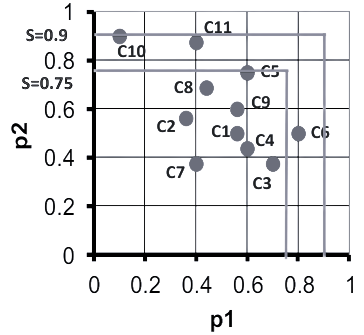
\includegraphics[width=0.75\linewidth]{images/iso.png} 
        \caption{Isometric}
    \end{subfigure}
    \begin{subfigure}{0.32\textwidth}
        \centering
        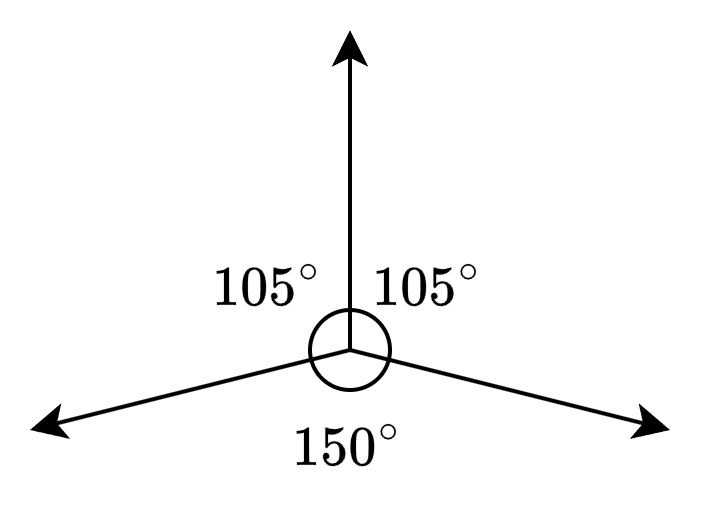
\includegraphics[width=0.75\linewidth]{images/dim.png}
        \caption{Dimetric}
    \end{subfigure}
    \begin{subfigure}{0.32\textwidth}
        \centering
        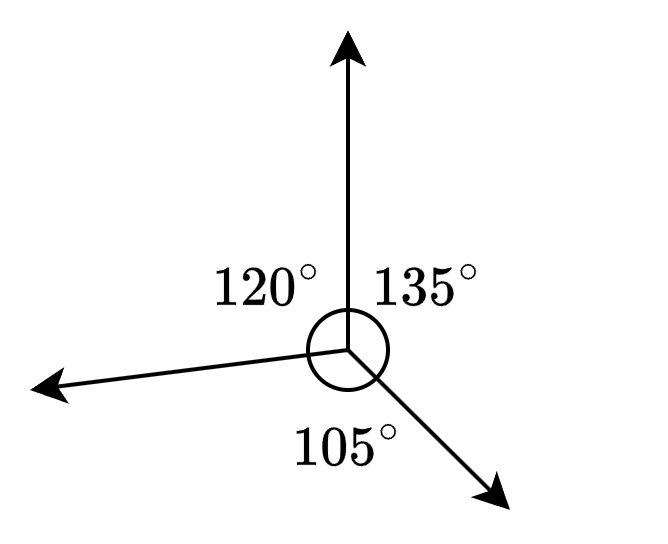
\includegraphics[width=0.75\linewidth]{images/tri.png} 
        \caption{Trimetric}
    \end{subfigure}
    \caption{Orthographic projections}
\end{figure}
A fundamental characteristic of axonometric projections is that they preserve the upward axis (the $y$-axis in our context) parallel to the vertical orientation of the screen.

\subsection{Oblique projections}
In oblique projections, rays are parallel but oblique in relation to the projection plane. 
Consequently, two of the three axes ($x$ and $y$) run parallel to the screen, while the third axis ($z$) is inclined at an angle to the other two.
The $z$-axis is commonly angled at $45^\circ$, $30^\circ$, or $60^\circ$, and it can be oriented in either direction.
The length of the $z$-axis can either match that of the other two axes or be halved. 
If the length is preserved, the projection is termed Cavalier; otherwise, it's referred to as Cabinet.

Oblique projections, valued for their simplicity in implementation using only integer arithmetic, found utility in some arcade and PC games.

These projections are achieved by applying a shear along the $z$-axis before the orthogonal projection:
\[\begin{bmatrix}
    \frac{1}{w} & 0 & 0 & 0 \\ 
    0 & -\frac{a}{w} & 0 & 0 \\ 
    0 & 0 & \frac{1}{n-f} & \frac{n}{n-f} \\ 
    0 & 0 & 0 & 1 
\end{bmatrix}\begin{bmatrix}
    1 & 0 & -\rho\cos(\alpha) & 0 \\ 
    0 & 1 & -\rho\sin(\alpha) & 0 \\ 
    0 & 0 & 1 & 0 \\ 
    0 & 0 & 0 & 1 
\end{bmatrix}\]
The shear factor determines the projection angle and whether it will be Cavalier or Cabinet. 
Specifically, it can be defined with respect to the axis angle, denoted as $\alpha$, and the corresponding reduction factor, denoted as $\rho$:
\begin{itemize}
    \item Cavalier: $\alpha=45^\circ$, $\rho=1$.
    \item Cabinet: $\alpha=45^\circ$, $\rho=0.5$.
\end{itemize}
    \section{Aitken method}

We have the following relation:
\[x^{(k+1)}-\alpha=\phi(x^{(k+1)})-\phi(\alpha)=\lambda_k\left( x^{(k+1)}-\alpha \right)\]
We know that $\lambda_k$ is the first derivative of $\phi$ at a certain point $\xi$. 
If we know $\lambda_k$, we can express $\alpha$ as: 
\[\alpha=\dfrac{\phi(x^{(k)})-\lambda_k x^{k}}{1-\lambda_k}\]
Additionally, the quantity:
\[A_k=\dfrac{\phi(\phi(x^{(k)}))-\phi(x^{(k)})}{\phi(x^{(k)})-x^{(k)}}\]
provides a good approximation of $\lambda_k$, so we can replace $\lambda_k$ with $A_k$. 
By substituting, we obtain the formula used in the Aitken method.
\begin{theorem}
    Let $\phi(x)=x-f(x)$ and $f(\alpha)$ be a simple zero. 
    Let $\phi^{(k)}$ converge to the first order to $\alpha$, then $\phi_A$ converge to the second order. 
    If $\phi(x)$ converges with order $p$ and $f(x)$ is still a simple zero, then $\phi_A$ converges with order $2p-1$. 
\end{theorem}
Occasionally, $\phi_A$ converges even when $\phi$ does not.

\subsection*{Algorithm}
\begin{algorithm}[H]
    \caption{Algorithm for the Aitken method}
        \begin{algorithmic}[1]
            \For {$k=0,1,\dots,n$}
                \State $x^{(k+1)}=x^{(k)}-\dfrac{\left[ \phi(x^{(k)})-x^{(k)} \right]^2}{\phi(\phi(x^{(k)}))-2\phi(x^{(k)})+x^{(k)}}$
                \If {stopping criterion is satisfied}
                    \State \Return $x^{(k+1)}$
                \EndIf
            \EndFor
        \end{algorithmic}
\end{algorithm} 
    \section{Dynamic modeling}

Dynamic modeling serves the purpose of providing methodologies for modeling interactions, the behavior of participants, and workflow within a system. 
This is achieved through various diagram types, including sequence diagrams, state machine diagrams, and activity diagrams. 
During the creation of these diagrams, certain objects become apparent.
 
A sequence diagram is established by following the flow of events outlined in the use case diagram. 
It represents objects engaged in a use case scenario using a directed acyclic graph notation. 
The fundamental rules for creating sequence diagrams include:
\begin{itemize}
    \item Every event involves both a sender and a receiver.
    \item The representation of the event is sometimes referred to as a message.
    \item The sender and receiver for each event must be identified.
\end{itemize}
\begin{figure}[H]
    \centering
    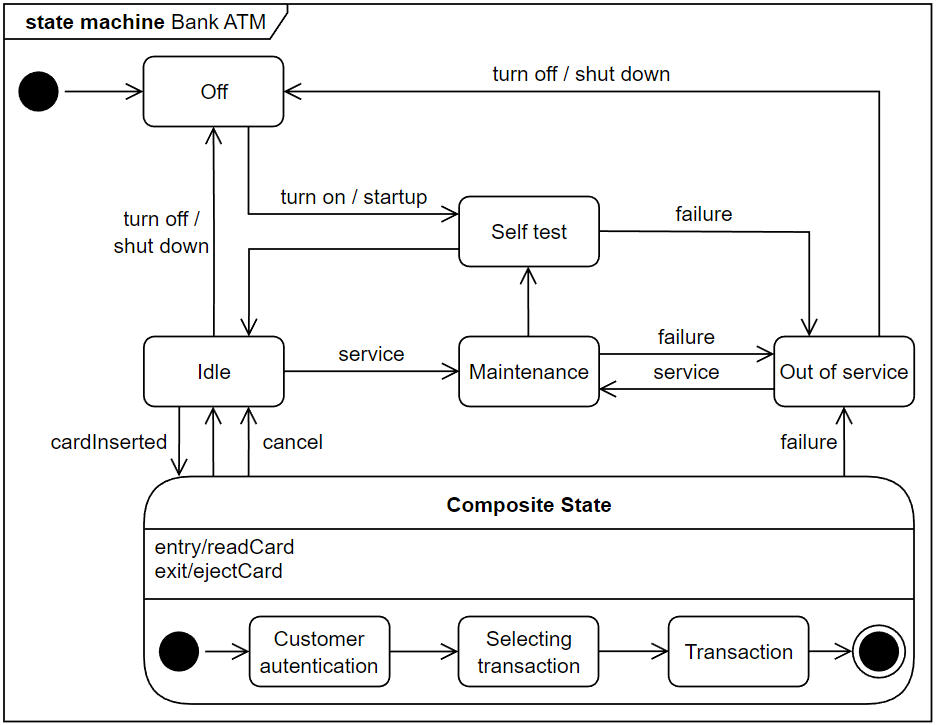
\includegraphics[width=0.5\linewidth]{images/state.png}
    \caption{Example of a state diagram}
\end{figure}
For effective dynamic modeling, it is crucial to construct models solely for classes exhibiting substantial dynamic behavior, considering only relevant attributes. 
Additionally, when deciding on actions and activities, one must account for the granularity of the application and strive to reduce notational complexity. 

    \chapter{Alloy}
    \section{Manufacturing company}

\begin{definition}[\textit{Information intensity}]
    Information intensity refers to the amount and complexity of information required in an organization's processes. 
\end{definition}
\noindent Generally, service industries require higher information intensity than manufacturing.
IT Intensity measures how well IT systems meet an organization's information processing needs. 
However, IT intensity can sometimes be greater in manufacturing than in services, depending on automation and digital integration.
\begin{definition}[\textit{Management inclination}]
    Management inclination reflects how much a company's leadership views IT as a strategic asset. 
\end{definition}
\noindent This varies based on factors like digital literacy, organizational culture, and company history.
Historically, manufacturing companies have adopted IT earlier, while service industries experienced a lag of around ten years.

\paragraph*{Drivers}
Several factors determine how IT intensive a company or industry can be:
\begin{enumerate}
    \item \textit{Structure of information processes}: the more structured and rule-based an activity is, the easier it is to automate using IT.
    \item \textit{Data volume}: the sheer amount of information that needs to be processed influences IT requirements.
    \item \textit{Operational frequency}: tasks that are repeated frequently benefit more from IT automation.
    \item \textit{Computational complexity}: simpler processes are easier to digitize and automate efficiently.
\end{enumerate}

\subsection{Manufacturing value chain}
Porter's value chain concept highlights how IT supports various business activities to create competitive advantages.
\begin{figure}[H]
    \centering
    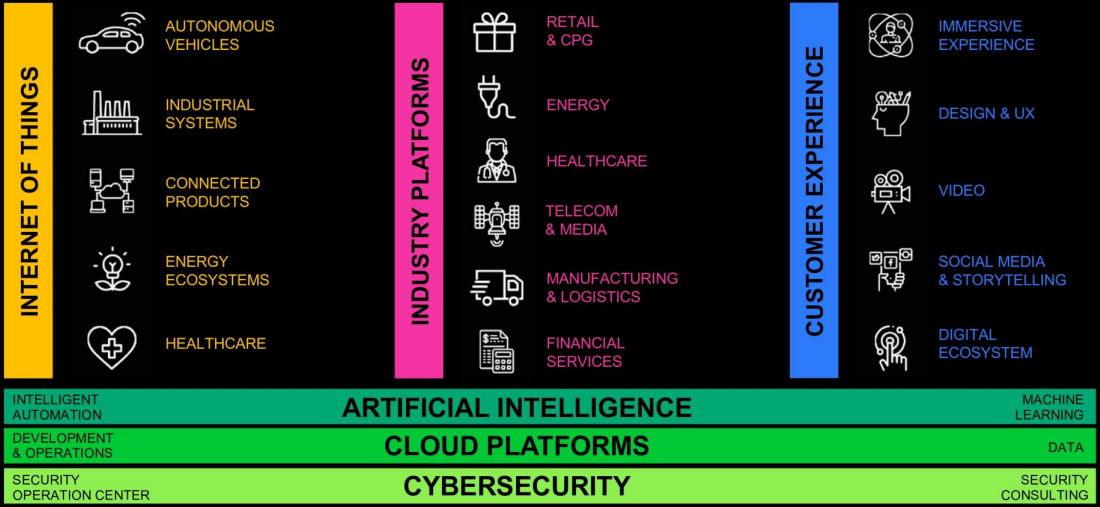
\includegraphics[width=0.75\linewidth]{images/bis2.png}
    \caption{Porter value chain}
\end{figure}

\paragraph*{Activity cycles}
Manufacturing involves continuous, iterative cycles that ensure efficiency and product quality. 
These cycles include:
\begin{enumerate}
    \item \textit{Development cycle}: focuses on designing and industrializing both products and production processes.
    \item \textit{Logistics cycle}: manages customer orders through:
        \begin{itemize}
            \item \textit{Procurement}: acquiring and handling materials, including reception, warehousing, and distribution to production plants.
            \item \textit{Production}: the physical transformation of raw materials into finished goods.
            \item \textit{Sales and distribution}: managing orders, external logistics, and post-sale services such as maintenance and customer support.
        \end{itemize}
\end{enumerate}

\subsection{Inter-functional information processes}
Inter-functional information processes play a key role in managing various aspects of production and operations within a company: 
\begin{enumerate}
    \item \textit{Order management process}: it manages the information regarding orders from order check in to post-sale services.
    \item \textit{Materials management process}: it manages the information regarding materials from outgoing orders towards suppliers to usage within transformation processes.
    \item \textit{Operations management process}: it manages the information regarding operations from materials dispatching to production plants to product delivery.
\end{enumerate}
\noindent These processes are interconnected across different products and divisions within the organization, making the information systems closely tied to the organizational structure. 
All production processes rely on the exchange of information across different functions. 
The use of inter-functional information extends beyond production and operations into planning and control processes. 
It also plays a vital role in administrative tasks.

\subsection{Production}
Companies may produce two types of goods: 
\begin{itemize}
    \item \textit{Standard production}: products have a finite set of predetermined features that can be changed to accommodate customer preferences. 
        In this case, companies produce according to a sales plan, before actual orders are received.
    \item \textit{Custom production}: products are designed according to customer requirements and then produced on demand.
\end{itemize}
\noindent While custom and standard production represent opposite ends of the production spectrum, there is a continuum between the two. 
Custom production is often seen in complex products, while standard production is associated with simpler goods. 
IT supports all production types, although its functionalities vary depending on the degree of customization or standardization in the production process.

\paragraph*{Product structure}
The product structure defines the hierarchical arrangement of components that make up a finished product. 
It ranges from individual components to larger product parts, outlining the relationships and dependencies between them.

\subsection{Information taxonomy}
Operational databases are organized to store various types of information that support the flow of activities within an organization. 
These can be categorized into three primary types: 
\begin{itemize}
    \item \textit{Transaction information}: describes the flow of operational activities, focusing on exchanges between different organizational units and external parties.
        It is the largest in terms of volumes. 
    \item \textit{Operation information}: details the objectives and expected results of operational activities. 
    \item \textit{Catalog information}: basic, static knowledge that exists independently of the flow of production activities. 
        It is quite complex and requires continuous updates and maintenance. 
        This information plays a key role in organizational learning.
\end{itemize}
\noindent Operations planning information is a key link between the operational and the executive portfolios.
Therefore, the level of detail of operational information is a driver of the efficiency of coordination inside an organization.
Operational information has intrinsic value as an organizational asset.
Its usefulness extends beyond internal operations, as it can sometimes be monetized or sold. 

\subsection{Information Technology integration}
Initially, IT functionalities were developed independently for each organizational function, without a comprehensive view of processes. 
The focus was on automating existing activities rather than supporting or re-engineering them to improve performance. 
Each function operated with separate data, and objectives were often misaligned, resulting in inefficiencies.

The traditional approach involved information being created at the start of a cycle and used later. 
However, to truly optimize organizational performance, a more proactive approach is needed. 
This involves using information at the executive level and integrating the various functions within an organization to create a unified view that enhances decision-making and operations.
There are two key approaches to IT integration:
\begin{itemize}
    \item \textit{Horizontal integration}: this refers to the integration of systems along the operating processes of an organization, specifically those that align with Porter's primary processes.
        This is done by the Computer Integrated Manufacturing (CIM), which is a system that supports the integration of manufacturing processes. 
    \item \textit{Vertical integration}: this focuses on connecting the operational portfolio with the executive portfolio. 
        This is done by the Material Requirements Planning (MRP), which ensures materials are available for production at the right time, helping optimize the production process and minimize waste.
\end{itemize}

\paragraph*{Computer Integrated Manufacturing}
CIM integrates various manufacturing processes. with the main objective of achieving an optimal scheduling and production resource management, which results in production efficiency. 
The main functionalities are: activities, workforce, plant, materials and quality management. 

\paragraph*{Materials Requirements Planning}
MRP is a production planning and inventory control system designed to manage manufacturing processes and ensure the availability of materials for production.
It emerged in the 1970s and 1980s with the aim of achieving flexibility and economies of scale through optimal planning. 
This is achieved with concurrent engineering (design and produce in parallel) and inside-out production processes (streamline production processes). 
MRP helps organizations achieve greater effectiveness by allowing them to respond more quickly to market demands while simultaneously benefiting from scale economies. 
    \section{Exercise 2}

An application permits the management of the bill of materials (BoM) of products. 
The BoM is the hierarchical description of a product in terms of the sub-products that comprise it. 
At each level but the last one, a product is associated with the components that make it, each with a quantity. 
The application allows the user to create BoMs.
A BoM is progressively assembled by attaching to a product its sub-products and specifying the number of units of sub-products that make one unit of the parent product. 
The editor accesses the HOME PAGE with the list of current BoMs and where s/he can create a new top level product and view the existing BOMs. 
The editor can add product-sub-products links to a product, modify the quantity of a product-sub-products link, delete a product or product-sub-products link. 
Products have an identifier, a name a description and a unit cost. 
An example of BoM is the following: 
\begin{figure}[H]
    \centering
    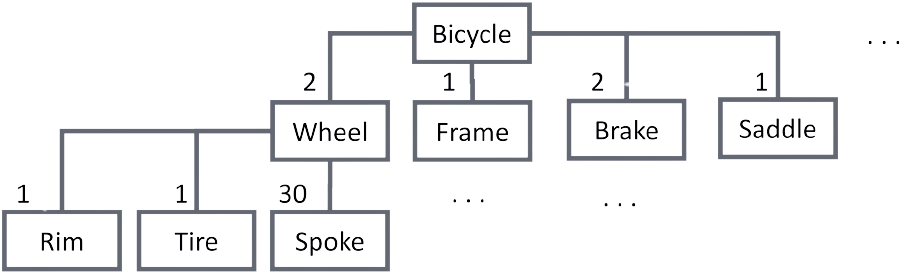
\includegraphics[width=1.0\linewidth]{images/BoM.png}
\end{figure}
The entity relationship model is the following:
\begin{figure}[H]
    \centering
    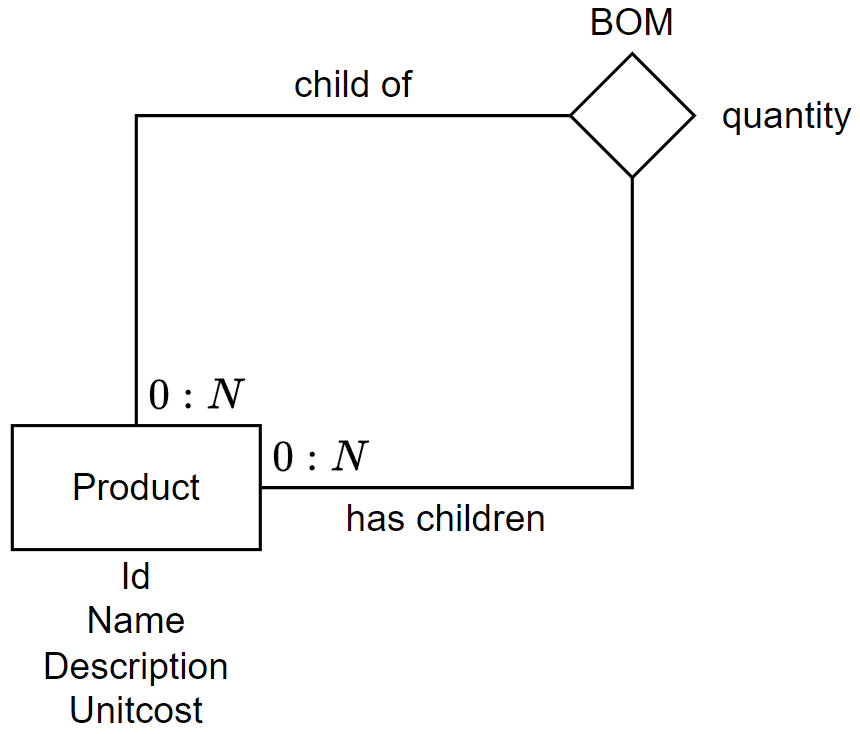
\includegraphics[width=0.5\linewidth]{images/e-r1.png}
\end{figure}
The relational schema DDL of the given database is: 
\begin{lstlisting}[style=SQL]
CREATE TABLE 'product' (
'id'            INT             NOT NULL AUTO_INCREMENT,
'unitcost'      INT             NOT NULL,
'name'          VARCHAR(45)     NOT NULL,
'description'   VARCHAR(45)     DEFAULT NULL,
PRIMARY KEY ('id')
) 
CREATE TABLE 'subparts' (
'father'        INT             NOT NULL,
'child'         INT             NOT NULL,
'quantity'      INT             NOT NULL,
PRIMARY KEY ('father','child'),
KEY 'childtoproduct_idx' ('child'),
CONSTRAINT 'childtoproduct' FOREIGN KEY ('child') REFERENCES 'product' ('id'),
CONSTRAINT 'fathertoproduct' FOREIGN KEY ('father') REFERENCES 'product' ('id')
)           
\end{lstlisting}
The relational model is: 
\begin{itemize}
    \item Product(\underline{id}, unitcost, name, description)
    \item Subparts(\underline{father}, \underline{child}, quantity)
\end{itemize}
Given the specifications, write the entity classes of the ORM mapping, including annotations for the attributes and for the relationships, fetch type of attributes and of relationships, and operation cascading policies for relationships (when not by default).

\subsection*{Solution}
Given the specifications write the entity classes of the ORM mapping, including annotations for the attributes and for the relationships, fetch type of attributes and of relationships, and operation cascading policies for relationships (when not by default). 
\begin{itemize}
    \item BoM: from father product to children product we have to use the annotations: 
        \begin{lstlisting}[style=Java]
@ManyToMany
        \end{lstlisting}
        From children product to father product we have to use these annotations: 
        \begin{lstlisting}[style=Java]
@ManyToMany
        \end{lstlisting}
        The owner of the relation is entity project. 
    \item 
\end{itemize}
The entity product is defined as:  
    \begin{lstlisting}[style=Java]
@Entity
@NamedQueries({
@NamedQuery(name = "BomProduct.findAll", query = "SELECT p FROM BomProduct p"),
@NamedQuery(name = "BomProduct.findAllTop", query = "SELECT p FROM BomProduct p WHERE p.fathers IS EMPTY") })

public class BomProduct implements Serializable {
    ...
    private static final long serialVersionUID = 1L;
    @Id @Column(name="id") @GeneratedValue(strategy = GenerationType.IDENTITY)
    private int id;
    private String description;
    private String name;
    private int unitcost;
    ...
    @ElementCollection(fetch = FetchType.EAGER)
    @CollectionTable(name = "subparts",joinColumns = @JoinColumn(name = "father"))
    @MapKeyJoinColumn(name = "child")
    @Column(name = "QUANTITY")
    private Map<BomProduct, Integer> subparts;

    @ManyToMany
    @JoinTable(name = "subparts",
            joinColumns = @JoinColumn(name = "child"),
            inverseJoinColumns = @JoinColumn(name ="father"))
    private List<BomProduct> fathers;
    ...            
}
    \end{lstlisting}
The better way is to make the many-to-many relationships with attributes a weak entity like in the following image. 
\begin{figure}[H]
    \centering
    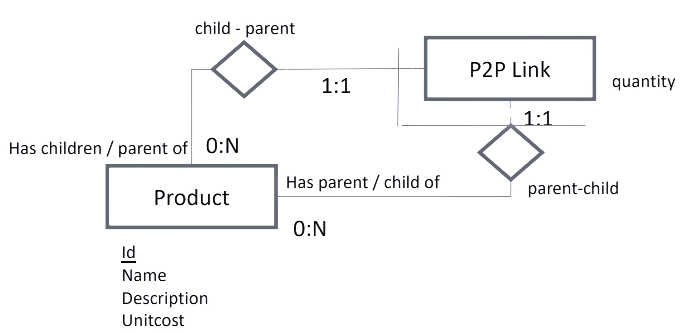
\includegraphics[width=0.5\linewidth]{images/BoMweak.png}
\end{figure}
The entity P2PLinkID is defined as:  
\begin{lstlisting}[style=Java]
@Embeddable
public class P2PLinkID implements Serializable {
    private static final long serialVersionUID = 1L;
    private int father;
    private int child;

    public P2PLinkID() { }

    public P2PLinkID(int father, int child) {
        super();
        this.father = father;
        this.child = child;
    }
    ...
}
\end{lstlisting}
The entity P2PLink is defined as:  
\begin{lstlisting}[style=Java]
@Entity
public class P2PLink implements Serializable {
    private static final long serialVersionUID = 1L;

    @EmbeddedId
    private P2PLinkID id;

    @ManyToOne
    @MapsId("father") // reference to the foreign key attribute
    @JoinColumn(name = "father")
    private BomProduct father;

    @ManyToOne
    @MapsId("child") // reference to the foreign key attribute
    @JoinColumn(name = "child")
    private BomProduct child;

    private int quantity;
    ...
}
\end{lstlisting}
The entity product is defined as:  
\begin{lstlisting}[style=Java]
@Entity
public class BomProduct implements Serializable {
    private static final long serialVersionUID = 1L;

    @Id @GeneratedValue(strategy = GenerationType.IDENTITY)
    private int id;
    private String description;
    private String name;
    private int unitcost;

    // getters setters and constructors

    @OneToMany(mappedby="father")
    private List<P2PLink> children;

    @OneToMany(mappedby="child")
    private List<P2PLink> fathers;
    ...
}
\end{lstlisting}
    \section{Exercise three}

The busy time of a virtual machine is 3 hours every 4 hours. 
Its utilization is 80\%, and on average, it is serving 5 jobs simultaneously. 
Determine:
\begin{enumerate}
    \item The system throughput.
    \item The average response time.
\end{enumerate}

\subsection*{Solution}
Given:
\[B=3\qquad T=4\qquad U=0.8 \qquad N=5\]
The utilization calculated from busy time and total time does not match the given utilization:
\[U=\dfrac{B}{T}=\dfrac{3}{4}=0.75\neq 0.8\]
The given data is inconsistent; therefore, this exercise cannot be solved.
    \section{Indices}
Search engines are designed to deliver results as quickly as possible, since any delay can impact user experience and attention. 
Responses must be returned within tenths of a second, so search engines are optimized for speed.

At the heart of this efficiency is the inverted index, which is the core data structure used by search engines to retrieve documents.

\subsection{Inverted indices}
An inverted index consists of posting lists, which map term IDs to document IDs. 
The basic idea is to create a mapping between terms and the documents that contain them, so that when a user searches for a term, the system can quickly find all the relevant documents.

To optimize for speed and reduce storage space, inverted indices often use integer compression algorithms, allowing for quick decompression and reducing the overall size of the index.

When calculating a retrieval function, the process typically involves joining posting lists. 
The documents within these lists are sorted by term frequency. 
This sorting allows for early termination of the results list computation, so irrelevant documents are discarded quickly.

\subsection{Positional indices}
In many cases, it's not just about whether a term appears in a document, but where it appears. 
To capture this, some indices maintain positional information, recording the exact locations of terms within documents. 
This allows for the calculation of proximity between query terms, which can be a useful indicator of relevance.

Moreover, the location of words within a webpage can influence their importance. 
In addition, certain statistically significant bigrams and trigrams are often identified and indexed separately. 
These are usually discovered using a technique like pointwise mutual information, which measures the association between terms. 
These bigrams or trigrams often have their own posting lists, as they can provide more context to queries.

\subsubsection{Crawlers}
To populate the index, web crawlers scour the web, following hyperlinks to discover and add new pages to the search engine's database. 
Effective crawling involves two main challenges:
\begin{itemize}
    \item \textit{Prioritizing URLs}: the crawler must decide which URLs to visit first based on factors like relevance and likelihood of finding fresh content.
    \item \textit{Re-visiting websites}: determining how often to revisit a website to check for updates is critical to ensuring that the index remains fresh and up to date.
\end{itemize}
\noindent At the scale of the web, crawlers must also be robust enough to handle different types of content, including dynamically generated pages.
Additionally, web crawlers must detect and manage duplicate content. Many different URLs may lead to the same content, and the crawler needs to ensure that it doesn't index the same page multiple times.

To manage these challenges, a distributed crawler architecture is typically used, with a centralized URL list to keep track of the pages the crawler needs to visit. 
Crawlers also respect robots.txt files, which are placed in the root directory of websites. 
These files tell crawlers which pages or sections of the site they are allowed to crawl and index, helping website owners manage how their content is indexed.

    \chapter{Software design}
    \section{Exercise one}

Consider the C program below, which is affected by a typical buffer overflow vulnerability.
\begin{verbnobox}[\verbarg]
#include <stdio.h>
#include <stdlib.h>
#include <string.h>

void vuln() {
    char buf[32];

    scanf("%s", buf);
    if (strncmp(buf, "Knight_King!", 12) != 0) {
        abort();
    }
}

int main(int argc, char** argv) {
    vuln();
}
\end{verbnobox}
\begin{enumerate}
    \item Assume that the program runs on the usual IA-32 architecture (32-bits), with the usual \texttt{cdecl} calling convention. 
        Also assume that the program is compiled without any mitigation against exploitation (ASLR is off, stack is executable, and stack canary is not present).
        Draw the stack layout when the program is executing the instruction at line seven, showing:
        \begin{itemize}
            \item Direction of growth and high-low addresses.
            \item The name of each allocated variable.
            \item The boundaries of frame of the function frames (\texttt{main} and \texttt{vuln}).
        \end{itemize}
        Show also the content of the caller frame.
    \item Write an exploit for the buffer overflow vulnerability in the above program. 
        Your exploit should execute the following simple shell code, composed only by four instructions: \texttt{0x12 0x34 0x56 0x78}.
        Write clearly all the steps and assumptions you need for the exploitation, and show the stack layout right after the execution of the \texttt{scanf()} during the program exploitation.
\end{enumerate}

\subsection*{Solution}
\begin{enumerate}
    \item To represent the stack layout described, we need to allocate space for the \texttt{buf} array, the saved EBP, and the saved EIP:
        \begin{figure}[H]
            \centering
            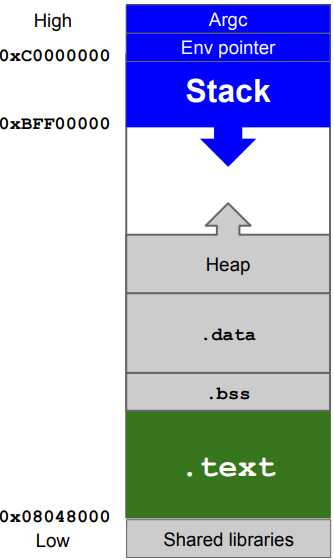
\includegraphics[width=0.5\linewidth]{images/stack.png}
        \end{figure}
    \item The stack in this case is: 
        \begin{figure}[H]
            \centering
            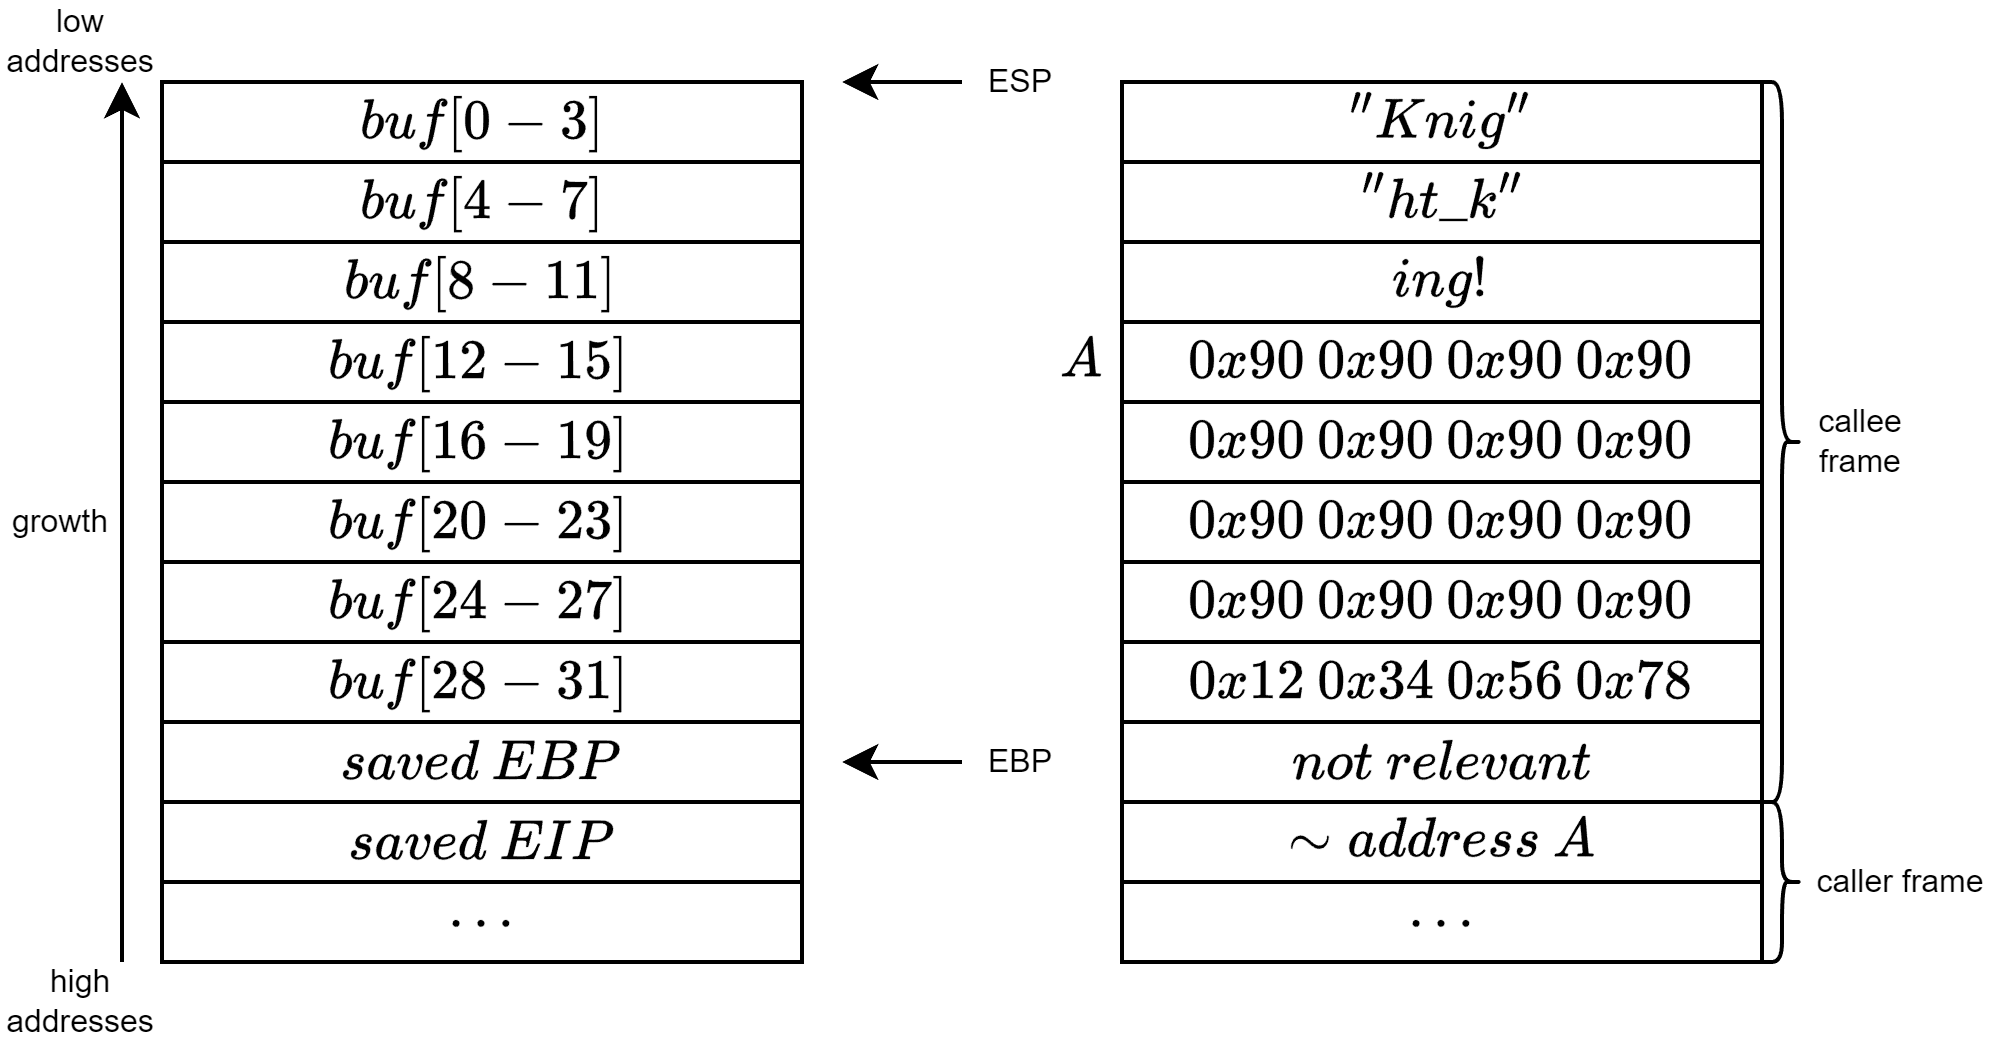
\includegraphics[width=0.75\linewidth]{images/stack1.png}
        \end{figure}
        In this layout:
        \begin{itemize}
            \item The first 16 bytes (four cells) are filled with no-operation instructions to avoid any unintended actions.
            The next 8 bytes (two cells) are reserved for the \texttt{buf} array.
            The following 4 bytes (one cell) are allocated for the saved EBP.
            The last 4 bytes (one cell) contain the address of the shell code.
        \end{itemize}
        The first twelve characters of \texttt{buf} are ensured to be different from "Knight\_King!" to avoid invoking \texttt{abort()}.
\end{enumerate}
    \section{Dependability principles}

Dependability is a critical consideration both during the design phase and during runtime operations.
During the design phase, it is essential to:
\begin{itemize}
    \item Analyze the system under development.
    \item Evaluate and measure its dependability properties.
    \item Make necessary modifications to the design as needed.
\end{itemize}
During runtime, the focus shifts to:
\begin{itemize}
    \item Detecting any malfunctions or failures that occur.
    \item Investigating and understanding the root causes of these issues.
    \item Taking appropriate reactive measures to address and mitigate the impact of the malfunctions.
\end{itemize}
Failures are commonplace in both the development and operational stages: while those in development should be averted, operational failures, being unavoidable due to the nature of system components, must be managed effectively. 
Design processes should factor in these potential failures to ensure that control and safety measures remain intact even when failures arise. 
Moreover, the effects of these failures should be predictable and deterministic rather than catastrophic.

Once upon a time, dependability was primarily a concern in safety-critical and mission-critical application domains like space exploration, nuclear facilities, and avionics. 
This was largely due to the significant cost associated with ensuring dependability, which was deemed acceptable only when absolutely necessary.
In non-critical systems, operational failures can lead to economic losses and damage to reputation, as seen in consumer products. 
However, in mission-critical systems such as satellites, automatic weather stations, surveillance drones, and unmanned vehicles, operational failures can result in serious or irreversible consequences for the mission at hand.
Safety-critical systems, on the other hand, pose a direct threat to human life if they fail during operation.
Examples include aircraft control systems, medical instrumentation, railway signaling, and nuclear reactor control systems.
    \section{Dependency}

To achieve higher performance within a given technology, it is crucial to extract more parallelism from the program. 
This involves detecting and resolving dependencies and scheduling instructions to maximize execution parallelism with the available resources.

Dependencies among instructions are key to determining the level of parallelism in a program. 
If two instructions are dependent on each other, they cannot execute simultaneously and must be executed sequentially or with limited overlap. 
There are three types of dependencies: name, data, and control dependencies.

\subsection{Name dependency}
A name dependency occurs when two instructions use the same register or memory location without any data flow between them.
There are two types of name dependencies between an instruction $i$ preceding instruction $j$:
\begin{itemize}
    \item \textit{Anti-dependence} (WAR): occurs when $j$ writes to a register or memory location that instruction $i$ reads. 
    \item \textit{Output dependence} (WAW): arises when both $i$ and $j$ write to the same register or memory location. 
\end{itemize}
Name dependencies differ from true data dependencies as there is no data flow between the instructions.

\paragraph*{Register Renaming}
If the names used in the instructions can be altered, the instructions do not conflict. 
Detecting dependencies through memory locations is more challenging since two addresses might refer to the same location but appear different. 
Register renaming is easier to implement and can be accomplished statically by the compiler or dynamically by the hardware.

\subsection{Data dependency}
Data dependencies can potentially create data hazards, but the actual hazard and the number of stalls required to eliminate it depend on the pipeline. 
There are three types of data hazards:
\begin{itemize}
    \item \textit{RAW hazards}: true data dependence.
    \item \textit{WAW hazards}: output dependence
    \item \textit{WAR hazards}: anti-dependence.
\end{itemize}
It is important to note that data dependencies are inherent to the program, while hazards are specific to the pipeline.

\subsection{Control dependency}
Control dependencies dictate the order of instruction execution, preserved by:
\begin{itemize}
    \item Executing instructions in program order to ensure that an instruction before a branch executes before the branch.
    \item Detecting control hazards to ensure that an instruction dependent on a branch is not executed until the branch direction is known.
\end{itemize}
While preserving control dependence is a simple way to maintain program order, it is not the most critical property that must be preserved for execution.
    \section{Scheduling}

Two essential properties must be maintained to ensure program correctness, typically achieved by preserving both data and control dependencies. 
The first is exception behavior, which ensures that any changes in the execution order of instructions do not affect how exceptions are triggered within the program. 
The second is data flow, which pertains to the actual movement of data values among instructions, ensuring that the correct results are produced and consumed.

There are two main strategies to support ILP: dynamic scheduling and static scheduling. 
Dynamic scheduling relies on hardware to identify and exploit parallelism within the program, while static scheduling depends on software to identify potential parallelism beforehand. 

\subsection{Dynamic scheduling}
Dynamic scheduling involves hardware reordering instruction execution to mitigate pipeline stalls while upholding data flow and exception behavior. 
The main advantages of this approach include handling cases where dependencies are unknown at compile time, simplifying compiler complexity, and facilitating efficient execution of compiled code on different pipeline architectures. 
However, these benefits come with costs such as a significant increase in hardware complexity, higher power consumption, and the potential for imprecise exceptions. 
In dynamic scheduling, instructions are fetched and issued in program order, but execution begins as soon as operands are available, potentially allowing out-of-order execution. 
This introduces the possibility of WAR and WAW data hazards and implies out-of-order completion unless a reorder buffer is present to ensure in-order completion.

\subsection{Static scheduling}
In static scheduling, compilers use sophisticated algorithms for code scheduling to harness ILP. 
While the ILP available within a basic block is often limited, significant performance improvements can be achieved by exploiting ILP across multiple basic blocks, transcending branches. 
Static scheduling involves the compiler detecting and resolving dependencies by reordering code to avoid conflicts. 
The compiler's output is typically dependency-free code, which is well-suited for architectures like Very Long Instruction Word (VLIW) processors. 
However, there are limits to ILP exploitation, including unpredictable branches, variable memory latency such as unpredictable cache misses, code size explosion, and increased compiler complexity.
    \section{Non-zero mean ARMA process}

Consider the ARMA process:
\[y(t)=\dfrac{C(z)}{A(z)}e(t) \qquad e(t)\sim WN(\mu,\lambda^2)\]
The expected value is:
\[\mathbb{E}\left[y(t)\right]=W(1)\mu=\bar{y}\]
Assuming the process is in canonical representation, we can express it as:
\[\begin{cases}
    \tilde{y}(t)=y(t)-\bar{y} \\
    \tilde{e}(t)=e(t)-\mu 
\end{cases} \rightarrow \tilde{y}(t)=W(z)\tilde{e}(t)\]
Applying the previously found prediction algorithm:
\begin{enumerate}
    \item Perform the long division.
    \item Take $\frac{F(z)}{A(z)}\tilde{e}(t)$. 
    \item Use the whitening filter.
\end{enumerate}
We obtain:
\[\hat{\tilde{y}}(t+k|t)=\dfrac{F(z)}{C(z)}\tilde{y}(t)\]

\paragraph*{Trivial solution}
To obtain the prediction for the original problem, we follow these steps:
\begin{itemize}
    \item Remove the mean from each data point: $\tilde{y}=y(t)-\bar{y}$. 
    \item Compute $\hat{\tilde{y}}(t+k|t)$. 
    \item Finally, the predicted value is given by: $\hat{y}(t+k|t)=\hat{\tilde{y}}(t+k|t)+\bar{y}$.
\end{itemize}

\paragraph*{Optimized solution}
Alternatively, we can integrate the computation of the correct predictor by modifying the formula.

Given that $y(t+k|t)=\tilde{y}(t+k|t)+\bar{y}$, we deduce:
\[\hat{y}(t+k|t)=\hat{\tilde{y}}(t+k|t)+\bar{y}=\dfrac{F(z)}{C(z)}\tilde{y}(t)+\bar{y}=\dfrac{F(z)}{C(z)}(y(t)-\bar{y})+\bar{y} \]
Asymptotically, $\dfrac{F(z)}{C(z)}\bar{y}$ tends to $\dfrac{F(1)}{C(1)}\bar{y}$:
\[\hat{y}(t+k|t)=\dfrac{F(z)}{C(z)}(y(t)-\bar{y})+\bar{y}=\dfrac{F(z)}{C(z)}y(t) + \left(1-\dfrac{F(1)}{C(1)}\right)\bar{y}\]
This represents the form of the predictor for an ARMA process with non-zero mean.
    \section{Exercise 6}

Consider the system: 
\[\mathcal{S}:y(t)=\dfrac{1}{3}y(t-1)+u(t-1)+\eta(t)+\dfrac{1}{2}\eta(t-1)\]
Here $\eta(t)\sim WN(0,1)$, $u(t)\sim WN(0,1)$ are two independent  White Noises
And the model: 
\[\mathcal{M}:y(t)=-ay(t-1)+bu(t-1)+e(t) \qquad e(t)\sim WN(0,\lambda^2)\]
Find the value of $\theta^\ast$ and $\lambda^{\ast 2}$. 

\subsection*{Solution}
The steps are: 
\begin{enumerate}
    \item Compute the predictor: 
        \[\hat{y}(t|t-1)=\dfrac{F(z)}{C(z)}y(t)+\dfrac{B(z)E(z)}{C(z)}u(t)=-\dfrac{a}{1}y(t-1)+\dfrac{bu(t-1)}{1}\]
    \item Compute the prediction error: 
        \[\varepsilon(t|t-1)=y(t)-\hat{y}(t|t-1)=y(t)+ay(t-1)-bu(t-1)\]
    \item Compute the variance of the prediction error: 
        \begin{align*}
            \bar{J}(\theta^\ast)    &=\text{Var}\left[\varepsilon(t)\right]\\   
                                    &=\mathbb{E}\left[ {\left(y(t)+ay(t-1)-bu(t-1)\right)}^2 \right] \\
                                    &=\left(1+a^{\ast 2}\right)\gamma_y(0)+b^{\ast 2}\gamma_u(0)+2a^\ast \gamma_y(1)-2b^\ast\mathbb{E}\left[y(t)u(t-1)\right]
        \end{align*}
    \item Derive with respect to the variables $a^\ast$ and $b^\ast$: 
        \[\dfrac{\partial\bar{J}(\theta^\ast)}{\partial a^\ast}=2a^\ast\gamma_y(0)+2\gamma_y(1)\]
        \[\dfrac{\partial\bar{J}(\theta^\ast)}{\partial b^\ast}=2b^\ast\gamma_y(0)+2\mathbb{E}\left[u(t-1)y(t)\right]\]
        We want a minimum, so we impose those derivatives to be null: 
        \[2a^\ast\gamma_y(0)+2\gamma_y(1)=0 \rightarrow a^\ast=-\dfrac{\gamma_y(1)}{\gamma_y(0)}\]
        \[2b^\ast\gamma_u(0)+2\mathbb{E}\left[u(t-1)y(t)\right]=0 \rightarrow b^\ast=\dfrac{\mathbb{E}\left[u(t-1)y(t)\right]}{\gamma_u(0)}\]
    \item We may now find the value of the covariance from the system $\mathcal{S}$: 
        \[\gamma_y(0)=\dfrac{69}{32}\]
        \[\gamma_y(1)=\dfrac{7}{32}\]
        As a result: 
        \[a^\ast=-\dfrac{\gamma_y(1)}{\gamma_y(0)}=-\dfrac{7}{69}\]
        \[b^\ast=\dfrac{\mathbb{E}\left[u(t-1)y(t)\right]}{\gamma_y(0)}=-\dfrac{\gamma_y(1)}{\gamma_y(0)}=1\]
    \item The value of $\lambda^{\ast 2}$ can be computed by substituting the value of $a^\ast$ and $b^\ast$ into the variance function: 
        \[\lambda^{\ast 2}=\left(1+a^{\ast 2}\right)\gamma_y(0)+b^{\ast 2}\gamma_u(0)+2a^\ast\gamma_y(1)-2b^\ast\mathbb{E}\left[y(t)u(t-1)\right]=1.134\]
        That is similar to the variance of the  White Noise, so the identification is good. 
\end{enumerate}

    \chapter{Documentation's structure}
    \section{Consulting}

Reply is a global network of over 150 specialized companies dedicated to helping organizations leverage cutting-edge technologies. 
Our mission is to drive innovation by enabling businesses to adapt to economic shifts and technological advancements, particularly those driven by the internet.
\begin{figure}[H]
    \centering
    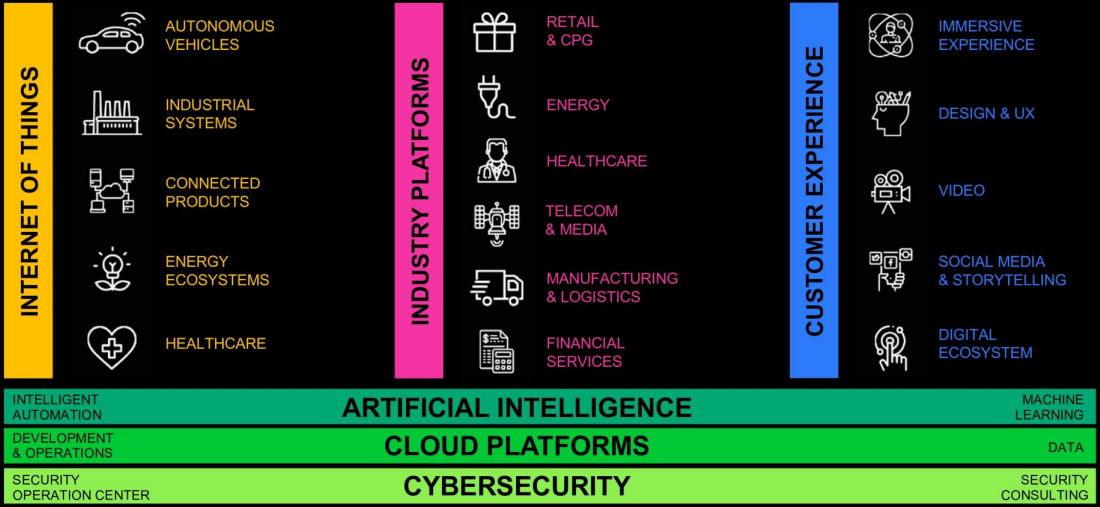
\includegraphics[width=0.5\linewidth]{images/bis2.png}
    \caption{Reply services}
\end{figure}
\noindent Reply provides end-to-end solutions for businesses looking to transform raw data into valuable insights. 
From data collection to advanced analytics, our approach ensures that companies can harness the full potential of their data.

In a consulting firm, professionals progress through several key roles, each with increasing responsibility and expertise:
\begin{enumerate}
    \item \textit{Consultant or analyst}: this is the entry-level position, where individuals focus on data analysis, research, and supporting senior consultants. 
        It's a foundational role that helps develop problem-solving, analytical, and research skills.
    \item \textit{Senior consultant or associate}: at this stage, professionals take on greater responsibility, leading specific project components and engaging more directly with clients.
        They begin to build deep expertise in a particular industry or domain while honing their client management skills.
    \item \textit{Manager}: managers oversee project teams, ensuring smooth project delivery while maintaining client relationships. 
        They are also involved in business development and sales. 
        This role emphasizes leadership, project management, and strategic client engagement.
    \item \textit{Senior manager}: with a broader scope, senior managers oversee multiple clients, contribute to business strategy, and play a key role in client acquisition. 
        Their focus shifts towards strategic thinking, high-level client management, and business development.
    \item \textit{Partner}: as part of the firm's leadership, partners are responsible for setting strategic direction, expanding business opportunities, and managing client relationships at the highest level.
        They bring extensive experience in business strategy, leadership, and client management.
\end{enumerate}

\subsection{Working models}
Consulting firms typically engage with clients through different contract models, depending on the project's nature and requirements.
\begin{itemize}
    \item \textit{Time and material}: in this model, the client pays based on the actual time spent and materials used, with an agreed hourly or daily rate for the resources employed. 
        This approach offers flexibility to adjust project requirements as work progresses and is well-suited for projects where specifications may evolve or are not fully defined at the outset. 
        However, budgeting can be challenging since the final cost depends on actual time and resources used.
    
    \item \textit{Turnkey}: the consulting provider takes full responsibility for delivering a complete and functional product or service. 
        The client receives the final result without managing the development process. 
        Costs and timelines are clearly defined, as the provider oversees all project phases. 
        This model requires minimal client involvement in day-to-day operations but offers limited flexibility to make changes once the project is underway.
        It is typically more expensive, as the provider factors in risks and contingencies.
    \item \textit{Service}: the client pays for a predefined set of consulting services, such as technical support, strategic guidance, or other specialized expertise. 
        This model allows clients to access specific skills without committing to a full project and is ideal for ongoing consultation or long-term support needs. 
        However, it may require clear agreements on service scope and expectations and is less suitable for projects with well-defined and temporary objectives.
\end{itemize}
\noindent The choice between these models depends on the project's complexity, flexibility needs, and budget considerations.
While time and material offers adaptability, turnkey ensures an end-to-end solution, and service contracts provide specialized expertise on demand.

\subsection{Key Performance Indicators}
\begin{definition}[\textit{Revenue}]
    The revenue is the total income generated by the company from its consulting services before any expenses are deducted.
\end{definition}
\noindent It is a key indicator of overall sales performance and business growth. 
In a consulting firm, revenue typically comes from client contracts and project fees.

\begin{definition}[\textit{Earning before tax}]
    Earning before tax is a financial metric that measures a company's profitability before accounting for income tax expenses.
\end{definition}
\noindent Earning before tax reflects the profit generated from core operations and other activities, such as investments or interest income, before taxes are deducted.

\begin{definition}[\textit{Cost on revenues}]
    cost on revenues is the ratio of costs directly associated with generating revenue, expressed as a percentage of total revenue.
\end{definition}
\noindent This metric helps assess how much of the revenue is consumed by costs such as consultant salaries, software tools, and travel expenses. 
A high cost-to-revenue ratio may indicate inefficiencies in service delivery or pricing strategies.

\begin{definition}[\textit{Unallocation}]
    Unallocation refers to staff who are not directly assigned to revenue-generating activities. 
\end{definition}
\noindent Monitoring unallocated costs is crucial for identifying inefficiencies and ensuring that expenses are properly distributed across projects and services.

\subsection{Project development}
The two main approaches used in project development are waterfall and agile, each with its own strengths and limitations.

\paragraph*{Waterfall}
The Waterfall model follows a sequential process, where each phase—analysis, design, development, testing, and implementation. 
Once a phase begins, changes to requirements are difficult to implement. 
This approach is best suited for projects with well-defined requirements from the start.
In consulting, waterfall is ideal for projects with stable and predetermined requirements, particularly in industries where compliance, documentation, and structured processes are essential.
\renewcommand*{\arraystretch}{1.5}
\begin{table}[!ht]
    \centering
    \begin{tabular}{|c|p{10cm}|}
    \hline
    \multicolumn{2}{|c|}{\textbf{Advantages}} \\ \hline
    \textit{Clear requirements}              & A well-defined project scope ensures a structured development process  \\ \hline
    \textit{Predictability}                  & Fixed timelines and structured phases make planning and resource allocation more manageable \\ \hline
    \textit{Comprehensive documentation}     & Each phase includes detailed documentation, providing a thorough project record \\ \hline
    \multicolumn{2}{|c|}{\textbf{Disadvantages}} \\ \hline
    \textit{Limited flexibility}             & Adapting to changes mid-project is challenging, making it less suitable for evolving requirements \\ \hline
    \textit{Delayed feedback}                & Since testing happens at the end, user feedback may come too late, requiring costly revisions \\ \hline
    \textit{Minimal client involvement}      & Limited collaboration during development can lead to misaligned expectations \\ \hline
\end{tabular}
\end{table}
\renewcommand*{\arraystretch}{1}

\paragraph*{Agile}
Agile follows an iterative and incremental approach, allowing for greater flexibility. 
Work is organized into sprints, each delivering a working product increment. 
Agile encourages continuous client collaboration and adapts easily to changing requirements.
In consulting, agile is well-suited for projects where requirements may evolve, or when quick, tangible results are needed.
\renewcommand*{\arraystretch}{1.5}
\begin{table}[!ht]
    \centering
    \begin{tabular}{|c|p{10cm}|}
    \hline
    \multicolumn{2}{|c|}{\textbf{Advantages}} \\ \hline
    \textit{Adaptability}                    & Changes can be accommodated at any stage, making Agile ideal for dynamic projects  \\ \hline
    \textit{Continuous feedback}             & Regular iterations ensure alignment with user needs and expectations \\ \hline
    \textit{Client collaboration}            & Ongoing client involvement fosters a more interactive and responsive development process\\ \hline
    \multicolumn{2}{|c|}{\textbf{Disadvantages}} \\ \hline
    \textit{Uncertain timeline}              &  Iterative cycles can introduce unpredictability, making planning and resource management more complex \\ \hline
    \textit{Minimal documentation}           & Agile prioritizes working software over documentation, which may be a drawback in highly regulated industries\\ \hline
    \textit{Scope creep}                     & Frequent changes and added features can lead to uncontrolled project expansion if not properly managed\\ \hline
\end{tabular}
\end{table}
\renewcommand*{\arraystretch}{1}
    \section{Data}

Data has become the foundation of decision-making, shaping industries and redefining business strategies. 
The journey of data-driven innovation can be divided into several key phases:

\begin{chronology}[5]{2010}{2025}{0.9\textwidth}
    \event[2012]{2015}{Big data}
    \event[2015]{2018}{Machine Learning}
    \event[2014]{2017}{Cloud computing}
    \event[2017]{2025}{Generative AI}
\end{chronology}

\paragraph*{Big data} 
Big data refers to the exponential growth of structured and unstructured data generated daily. 
It brought new challenges in storage, management, and analysis but also unlocked vast opportunities for business intelligence.
\renewcommand*{\arraystretch}{1.5}
\begin{table}[H]
    \centering
    \begin{tabular}{|l|l|}
    \hline
    \textbf{Technology} & Hadoop, Hive, Impala, Cloudera                                           \\ \hline
    \textbf{Key impact} & Data-driven decision-making, process optimization, competitive advantage \\ \hline
    \end{tabular}
\end{table}
\renewcommand*{\arraystretch}{1}

\paragraph*{Machine Learning}
Machine Learning marked the next stage of data evolution, enabling computers to learn patterns and make decisions without explicit programming. 
Machine Learning applications expanded rapidly, offering predictive insights and automation capabilities.
\renewcommand*{\arraystretch}{1.5}
\begin{table}[H]
    \centering
    \begin{tabular}{|l|l|}
    \hline
    \textbf{Technology} & Neural Networks, Deep Learning, Reinforcement Learning, Clustering                                  \\ \hline
    \textbf{Key impact} & Advanced automation, improved predictions, enhanced decision-making \\ \hline
    \end{tabular}
\end{table}
\renewcommand*{\arraystretch}{1}

\paragraph*{Cloud Computing}
Cloud computing revolutionized data storage and processing by providing scalable, cost-effective solutions over the internet. 
Businesses gained access to flexible computing power, reducing infrastructure constraints.
\renewcommand*{\arraystretch}{1.5}
\begin{table}[H]
    \centering
    \begin{tabular}{|l|l|}
    \hline
    \textbf{Technology} & AWS, Google Cloud Platform, Microsoft Azure                                 \\ \hline
    \textbf{Key impact} & Scalability, cost reduction, innovation acceleration \\ \hline
    \end{tabular}
\end{table}
\renewcommand*{\arraystretch}{1}

\paragraph*{Generative Artificial Inteligence}
Generative AI represents the latest frontier, where AI systems exhibit human-like understanding, learning, and application of knowledge across diverse domains.
Its potential is reshaping industries and redefining human-technology interaction.
\renewcommand*{\arraystretch}{1.5}
\begin{table}[H]
    \centering
    \begin{tabular}{|l|l|}
    \hline
    \textbf{Technology} & Large Language Models, synthetic data, Retrieval-Augmented Generation                                 \\ \hline
    \textbf{Key impact} & Creative automation, enhanced productivity, AI-driven decision making \\ \hline
    \end{tabular}
\end{table}
\renewcommand*{\arraystretch}{1}

\begin{figure}[H]
    \centering
    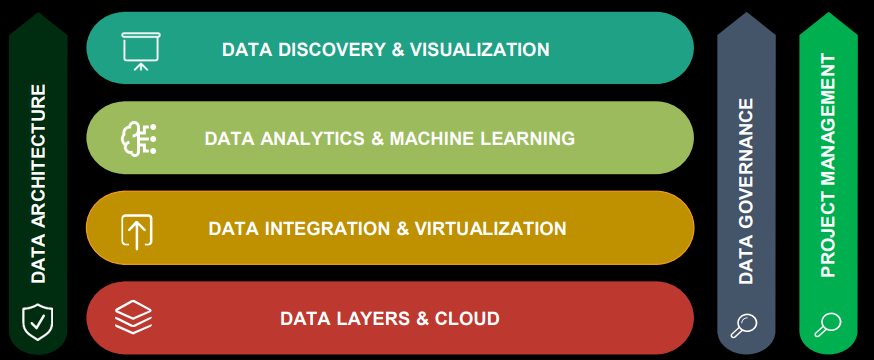
\includegraphics[width=0.5\linewidth]{images/bis3.png}
    \caption{Data framework}
\end{figure}


\subsection{Data job roles}

\paragraph*{Data and Cloud architect}
Data architects design comprehensive data infrastructures based on business objectives, ensuring seamless data integration and optimal storage solutions. 
Cloud Architects specialize in designing scalable, cloud-based architectures to support modern data needs.

\paragraph*{Data engineer}
Data engineers build and maintain the systems required for collecting, processing, and storing data. 
They design ETL pipelines, work with big data technologies, and ensure that raw data is transformed into a usable format.

\paragraph*{Data analyst}
Data analysts interpret and analyze data to provide actionable insights. 
They clean datasets, perform statistical analysis, and create visualizations to support business strategies and decision-making.

\paragraph*{Data scientist}
Data scientists develop machine learning models and apply advanced analytics to uncover patterns and predictions from complex datasets. 
They work with programming languages like Python and utilize AI-driven techniques for deeper insights.

\paragraph*{Data privacy and security specialist}
Data privacy officers ensure compliance with data protection regulations (e.g., GDPR), while security officers implement safeguards to protect organizational data from cyber threats and breaches.

\subsection{Data storage}
\begin{figure}[H]
    \centering
    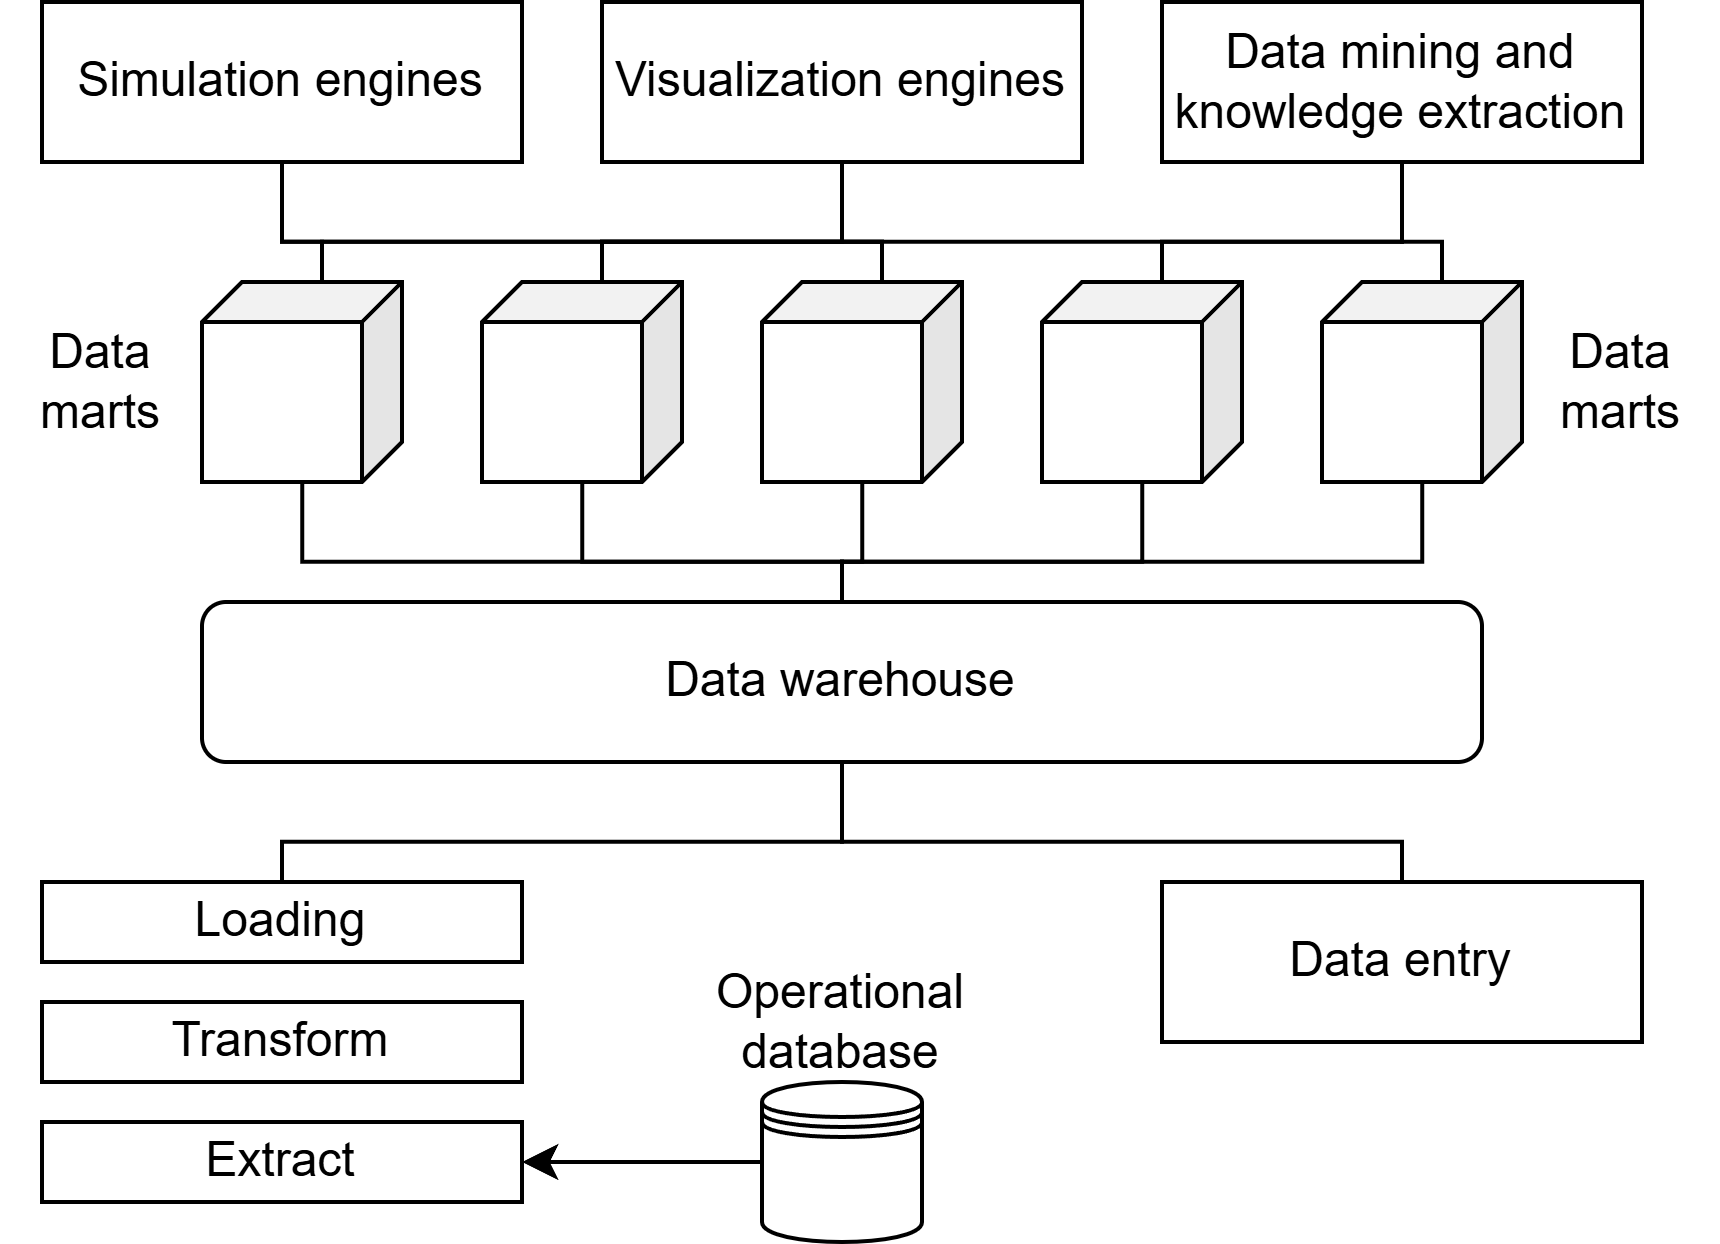
\includegraphics[width=0.5\linewidth]{images/bis4.png}
    \caption{Data architecture}
\end{figure}
The data architecture is structured as follows:
\begin{enumerate}
    \item \textit{Source layer}: this is where raw data originates, coming from operational systems, websites, e-commerce platforms, and other sources.
    \item \textit{Data ingestion}: as data is collected from the source, it undergoes transformations to make it usable within the data platform. 
        This step ensures that the data is properly formatted for analysis, enabling it to generate value for businesses.
    \item \textit{Data platform}: this is where the core data analysis happens. 
        Given the large volume of data, robust systems are needed to process it effectively. 
        The data refinement process follows a tiered approach:
        \begin{itemize}
            \item \textit{Bronze layer}: raw ingested data.
            \item \textit{Silver layer}: data undergoes Extract, Transform, Load processing.
            \item \textit{Gold layer}: fully analyzed and user-friendly data, optimized for reporting and decision-making.
        \end{itemize}
    \item \textit{Machine Learning} (optional): in this stage, advanced analytics and machine learning techniques extract valuable insights and patterns from the processed data.
    \item \textit{Data consumer}: the final processed data and insights are presented to end users or integrated into other applications, often in a visualization tool like Tableau.
\end{enumerate}
\begin{definition}[\textit{Data warehouse}]
    A data warehouse is a centralized repository that stores large volumes of structured data from various sources within an organization.
\end{definition}
\noindent Unlike transactional databases, which prioritize real-time operations, data warehouses are designed for analytical queries and historical data analysis. 
They facilitate reporting, business intelligence, and decision-making by providing a consolidated and structured view of organizational data.
\begin{definition}[\textit{Data lake}]
    A data lake is a scalable repository that allows organizations to store vast amounts of raw, structured, semi-structured, and unstructured data.
\end{definition}
\noindent Unlike a data warehouse, a data lake does not impose a schema on the data upon ingestion. 
Instead, it retains data in its original format until it is needed for processing or analysis.
While data lakes provide flexibility for advanced analytics and machine learning, they require careful governance and security measures to maintain data quality.

\paragraph*{Data lakehouse}
Organizations often integrate data warehouses and data lakes as part of a comprehensive data strategy, leveraging the strengths of both approaches:
\begin{itemize}
    \item \textit{Data integration}: raw data is ingested into the data lake, preserving its original format and serving as a staging area before further processing.
    \item \textit{Data transformation}: Extract, Transform, Load processes can take place in both the data lake and data warehouse. 
        Structured data required for immediate reporting is transformed and stored in the warehouse, while raw and unstructured data remains in the lake for exploratory analysis.
\end{itemize}
\begin{definition}[\textit{Data lakehouse}]
    A data lakehouse is a hybrid approach that combines data warehouses and data lakes.
\end{definition}
\noindent It provides a unified architecture that supports structured, semi-structured, and unstructured data, enabling both traditional business intelligence and modern machine learning workflows.
\begin{definition}[\textit{Polyglot persistence}]
    Polyglot persistence refers to the practice of using multiple types of data storage technologies and databases within a single system. 
\end{definition}
\noindent Instead of relying on a single storage solution, organizations select the best-suited technology for each specific data type and use case, optimizing performance and scalability across different applications.

\subsection{Data mesh}
\begin{definition}[\textit{Data mesh}]
    Data Mesh is a modern approach to analytical data architecture that treats data as a product.
\end{definition}
\noindent It is domain-driven, meaning that data ownership is distributed among teams that have the best understanding of their data and how it is used.

The key idea behind Data Mesh is that no one understands data better than its owner. 
Instead of relying on a centralized data team, Data Mesh distributes data responsibilities to domain-specific teams. 
Each domain aligns with a business function rather than specific applications or systems.
Each domain manages its own data pipelines within a shared infrastructure and provides access to domain-specific data and functionalities via APIs.

Data Mesh aims to improve the way organizations handle data by focusing on three key objectives:
\begin{itemize}
    \item \textit{Business enablement}: democratizing data with a self-service approach, reducing dependence on IT.
    \item \textit{Data management}: simplifying data processing, organization, and governance.
    \item \textit{Organizational efficiency}: facilitating seamless exchange of data products between producers and consumers.
\end{itemize}

\renewcommand{\arraystretch}{1.5}
\begin{table}[!ht]
    \centering

    \begin{tabular}{|l|p{4cm}|p{4cm}|p{4cm}|}
        \hline
        \textbf{Feature} & \textbf{Data warehouse} & \textbf{Data lake} & \textbf{Data mesh} \\ \hline
        \textit{Centralization} & Centralized & Centralized & Decentralized \\ \hline
        \textit{Data structure} & Structured & Unstructured & Both \\ \hline
        \textit{Use cases} & Reporting & Advanced analytics & Data product \\ \hline
        \textit{Integration} & Data lake & Data warehouse & Autonomous \\ \hline
        \textit{Flexibility} & No & No & Yes \\ \hline
    \end{tabular}
\end{table}
\renewcommand{\arraystretch}{1}

\subsection{Data governance}
Data governance is the framework that defines how an organization manages its data to ensure accuracy, security, and compliance. 
It encompasses processes, roles, policies, standards, and metrics to optimize data usage, enabling a company to become truly data-driven.
\begin{figure}[H]
    \centering
    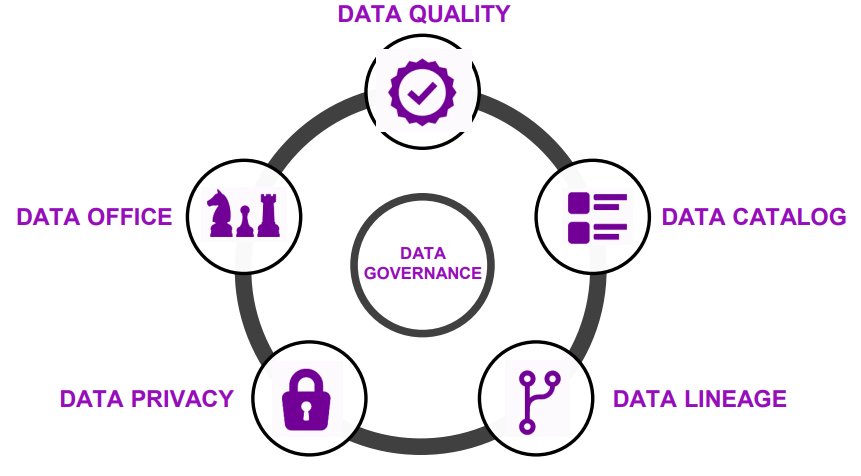
\includegraphics[width=0.5\linewidth]{images/bis5.png}
    \caption{Data governance pillars}
\end{figure}
Data governance relies on several foundational elements: 
\begin{itemize}
    \item \textit{Data quality}: ensures that information is accurate, reliable, and well-maintained. 
        It involves defining validation rules, monitoring quality at various stages, and using analytics to assess reliability. 
        AI-powered techniques, such as machine learning-driven validation, further enhance the integrity of data.
    \item \textit{Data catalog}: helps organizations manage and understand their data assets. 
        It integrates metadata from diverse sources such as databases, cloud platforms, ETL processes, and business intelligence tools. 
        By maintaining a structured data dictionary for IT teams and a data glossary for business users, companies can enhance collaboration and ensure consistency in data interpretation. 
        AI-driven search capabilities enable efficient metadata discovery and classification, supporting better knowledge sharing across the organization.
    \item \textit{Data lineage}: tracks the entire lifecycle of data, from its origin to its final destination. 
        By mapping transformations and interdependencies, it provides insights into how data moves through systems. 
        This capability is essential for assessing the impact of changes, optimizing service requests, and ensuring regulatory compliance. 
        Understanding data lineage also plays a crucial role in data protection, allowing organizations to pinpoint storage locations and enforce appropriate security measures.
    \item \textit{Data privacy}: focuses on the identification and safeguarding of sensitive information. 
        Effective privacy solutions assess risks, monitor data movement, and implement preventive measures to mitigate breaches. 
        Encryption, data masking, and access control policies ensure compliance with regulatory requirements while maintaining confidentiality. 
        Continuous analysis of data risks and proactive remediation strategies strengthen an organization's ability to protect its assets.
    \item \textit{Data office}: plays a key role in overseeing data governance initiatives. 
        Beyond technological solutions, governance efforts require clearly defined roles, responsibilities, and standardized management processes. 
        The Data Office establishes documentation templates, development guidelines, and monitoring frameworks to ensure governance policies are consistently applied.
\end{itemize}
\noindent Organizations rely on specialized technology platforms such as Informatica and Collibra to implement robust data governance strategies. 
These tools provide comprehensive capabilities for managing data quality, cataloging metadata, tracking lineage, and ensuring privacy. 
However, technology alone is not enough: effective governance requires a combination of tools, processes, and dedicated personnel within a structured Data Office.

Beyond compliance and data management, data governance serves as a strategic enabler for organizations. 
By establishing strong governance practices, companies can leverage their data assets more effectively, leading to innovations in areas such as data as a service and data monetization.

\paragraph*{Data monetization}
Data monetization transforms data into a valuable business asset by extracting insights that can be sold or leveraged for competitive advantage. 
High-quality, well-governed data enables businesses to identify new revenue opportunities, enhance market positioning, and strengthen partnerships.
With the right governance framework in place, organizations can shift from merely being data-driven to becoming proactive data providers, delivering insights that generate tangible business value.
    \section{Norm of matrices}

\begin{definition}
    The \emph{p-norm} of a matrix $A$ is defined as: 
    \[\left\lVert A \right\rVert_p=\max_{x \neq 0}{\left( \dfrac{\left\lVert A_x \right\rVert_p}{\left\lVert x \right\rVert_p} \right)}=
    \max_{\left\lVert x \right\rVert_p=1}{\left( \left\lVert A_x \right\rVert_p \right)}\]
\end{definition}
The most used matrix's norms are: 
\begin{itemize}
    \item $\left\lVert A \right\rVert_1=\max_{i}{\sum_{i=1}^{n}{\left\lvert a_{ij} \right\rvert}}$
    \item $\left\lVert A \right\rVert_2=\left\lVert A \right\rVert=\sqrt{\sum{\lambda_{max}{\left( A^TA \right)}}}$
    \item $\left\lVert y \right\rVert_A=\sqrt{y^TAy}$
    \item $\left\lVert A \right\rVert_{\infty}=\max_{j}{\sum_{j=1}^{n}{\left\lvert a_{ij} \right\rvert}}$
\end{itemize}
\begin{proposition}
    If the matrix $A$ is symmetric positive definite we have that: 
    \[\left\lVert A \right\rVert_2=\lambda_{max}\]
\end{proposition}

\end{document}